% Options for packages loaded elsewhere
\PassOptionsToPackage{unicode}{hyperref}
\PassOptionsToPackage{hyphens}{url}
\documentclass[
  ignorenonframetext,
]{beamer}
\newif\ifbibliography
\usepackage{pgfpages}
\setbeamertemplate{caption}[numbered]
\setbeamertemplate{caption label separator}{: }
\setbeamercolor{caption name}{fg=normal text.fg}
\beamertemplatenavigationsymbolsempty
% remove section numbering
\setbeamertemplate{part page}{
  \centering
  \begin{beamercolorbox}[sep=16pt,center]{part title}
    \usebeamerfont{part title}\insertpart\par
  \end{beamercolorbox}
}
\setbeamertemplate{section page}{
  \centering
  \begin{beamercolorbox}[sep=12pt,center]{section title}
    \usebeamerfont{section title}\insertsection\par
  \end{beamercolorbox}
}
\setbeamertemplate{subsection page}{
  \centering
  \begin{beamercolorbox}[sep=8pt,center]{subsection title}
    \usebeamerfont{subsection title}\insertsubsection\par
  \end{beamercolorbox}
}
% Prevent slide breaks in the middle of a paragraph
\widowpenalties 1 10000
\raggedbottom
\AtBeginPart{
  \frame{\partpage}
}
\AtBeginSection{
  \ifbibliography
  \else
    \frame{\sectionpage}
  \fi
}
\AtBeginSubsection{
  \frame{\subsectionpage}
}
\usepackage{iftex}
\ifPDFTeX
  \usepackage[T1]{fontenc}
  \usepackage[utf8]{inputenc}
  \usepackage{textcomp} % provide euro and other symbols
\else % if luatex or xetex
  \usepackage{unicode-math} % this also loads fontspec
  \defaultfontfeatures{Scale=MatchLowercase}
  \defaultfontfeatures[\rmfamily]{Ligatures=TeX,Scale=1}
\fi
\usepackage{lmodern}
\ifPDFTeX\else
  % xetex/luatex font selection
\fi
% Use upquote if available, for straight quotes in verbatim environments
\IfFileExists{upquote.sty}{\usepackage{upquote}}{}
\IfFileExists{microtype.sty}{% use microtype if available
  \usepackage[]{microtype}
  \UseMicrotypeSet[protrusion]{basicmath} % disable protrusion for tt fonts
}{}
\makeatletter
\@ifundefined{KOMAClassName}{% if non-KOMA class
  \IfFileExists{parskip.sty}{%
    \usepackage{parskip}
  }{% else
    \setlength{\parindent}{0pt}
    \setlength{\parskip}{6pt plus 2pt minus 1pt}}
}{% if KOMA class
  \KOMAoptions{parskip=half}}
\makeatother
\usepackage{longtable,booktabs,array}
\newcounter{none} % for unnumbered tables
\usepackage{calc} % for calculating minipage widths
\usepackage{caption}
% Make caption package work with longtable
\makeatletter
\def\fnum@table{\tablename~\thetable}
\makeatother
\usepackage{graphicx}
\makeatletter
\newsavebox\pandoc@box
\newcommand*\pandocbounded[1]{% scales image to fit in text height/width
  \sbox\pandoc@box{#1}%
  \Gscale@div\@tempa{\textheight}{\dimexpr\ht\pandoc@box+\dp\pandoc@box\relax}%
  \Gscale@div\@tempb{\linewidth}{\wd\pandoc@box}%
  \ifdim\@tempb\p@<\@tempa\p@\let\@tempa\@tempb\fi% select the smaller of both
  \ifdim\@tempa\p@<\p@\scalebox{\@tempa}{\usebox\pandoc@box}%
  \else\usebox{\pandoc@box}%
  \fi%
}
% Set default figure placement to htbp
\def\fps@figure{htbp}
\makeatother
\setlength{\emergencystretch}{3em} % prevent overfull lines
\providecommand{\tightlist}{%
  \setlength{\itemsep}{0pt}\setlength{\parskip}{0pt}}
% Slide layout defaults for warning-clean scientific decks.
\usepackage{etoolbox}
\IfFileExists{xurl.sty}{\usepackage{xurl}}{}
\IfFileExists{seqsplit.sty}{\usepackage{seqsplit}}{\newcommand{\seqsplit}[1]{#1}}
\protected\def\breakseq#1{\seqsplit{#1}}
\protected\def\breaktt#1{\begingroup\ttfamily\seqsplit{#1}\endgroup}
\setlength{\emergencystretch}{6em}
\tolerance=5000
\hbadness=10000
\hfuzz=1pt
\setlength{\tabcolsep}{2pt}
\AtBeginEnvironment{longtable}{\tiny\renewcommand{\arraystretch}{0.86}\setlength{\tabcolsep}{1pt}}
\AtBeginEnvironment{tabular}{\tiny\renewcommand{\arraystretch}{0.86}\setlength{\tabcolsep}{1pt}}

% Natbib and cross-reference fallbacks — slides don't load natbib
% or cleveref, but combined-PDF manuscript prose may emit these
% commands. The fallback renders citations as a bracketed key list
% and cross-references as detokenized labels so slides don't fail on
% undefined control sequences or raw underscores. \providecommand is
% a no-op if packages load later.
\providecommand{\citep}[1]{[#1]}
\providecommand{\citet}[1]{#1}
\providecommand{\citealp}[1]{#1}
\providecommand{\citeauthor}[1]{#1}
\providecommand{\citeyear}[1]{#1}
\providecommand{\cref}[1]{\texttt{\detokenize{#1}}}
\providecommand{\Cref}[1]{\texttt{\detokenize{#1}}}
\usepackage{bookmark}
\IfFileExists{xurl.sty}{\usepackage{xurl}}{} % add URL line breaks if available
\urlstyle{same}
% fallback for those not using the hyperref driver hyperxmp:
\makeatletter
\@ifundefined{xmpquote}{\newcommand{\xmpquote}[1]{#1}}{}
\makeatother
\hypersetup{
  hidelinks,
  pdfcreator={LaTeX via pandoc}}

\author{\texorpdfstring{}{}}
\date{}

\begin{document}

\section{Results: what resolved and what stayed
bounded}\label{results-what-resolved-and-what-stayed-bounded}

\begin{frame}[fragile,allowframebreaks]{Results: what resolved and what
stayed bounded}
Numbers below are token-injected by
\breaktt{src/ntqr\_allotment/manuscript\_variables.py} from the artifact
named in each section: \breaktt{sweep\_aggregated.csv} for strategy and
size summaries, \breaktt{independence\_sweep.csv} for tolerance,
\breaktt{postdoc\_panel\_results.json} and
\breaktt{postdoc\_panel\_alignment.json} for the live Gemma
reviewer-panel companion, \breaktt{power\_analysis.csv} /
\breaktt{sweep\_results.json} for design budgets, and
\breaktt{alarm\_timings.csv} for alarm timing. None are hand-transcribed.
Errors are mean EIE recovery error against the supervised oracle,
aggregated over 96 seeds in the active sweep profile.

This section adjudicates the five hypotheses from the Introduction. H1,
H3, and H5 each resolve in one subsection. H2 and H4 are addressed in
two stages: first against the baseline grid (where, by construction,
both are design-limited because the baseline judges err independently),
then resolved together by the composition-coupled confound. Remaining
subsections report supporting diagnostics. The Discussion returns the
per-hypothesis verdicts.
\end{frame}

\begin{frame}[fragile,allowframebreaks]{Synthetic deterministic results:
controlled spine for H1-H4}
\protect\phantomsection\label{synthetic-deterministic-results-controlled-spine-for-h1-h4}
The synthetic results are generated from seeded populations and corpora
with a known oracle. They support strategy, regime, tolerance,
power-budget, alarm, and diagnostic claims for the active deterministic
profile only. Throughout, a \emph{regime} is one (expert-stringency ×
bias-spread × panel-size) cell of the sweep grid (sixteen cells in the
active profile); contrasts are evaluated cell by cell and averaged only
where the text says so.

\begin{block}{Formation strategy sets the recovery floor}
\protect\phantomsection\label{formation-strategy-sets-the-recovery-floor}
\textbf{H1 (formation strategy is the dominant lever).} The strategies
do not fan out into a graded four-way ranking; instead one rule stands
far apart and the other three collapse together (\breakseq{[@fig:ranking]}).
Competence-first selection recovers at mean EIE error 0.037 --- roughly
a quarter of the error of any other rule --- while representative
sortition, random selection, and single-bloc ideological selection are
\textbf{statistically indistinguishable from one another}, clustered at
0.147--0.148:

{\def\LTcaptype{none} % do not increment counter
\begin{longtable}[]{@{}lll@{}}
\toprule\noalign{}
Strategy & Mean EIE error & 95\% CI \\
\midrule\noalign{}
\endhead
expertise threshold (far best) & 0.037 & ±0.003 \\
representative sortition & 0.147 & ±0.014 \\
random selection & 0.148 & ±0.014 \\
single-bloc ideological selection & 0.148 & ±0.015 \\
\bottomrule\noalign{}
\end{longtable}
}

\begin{figure}
\centering
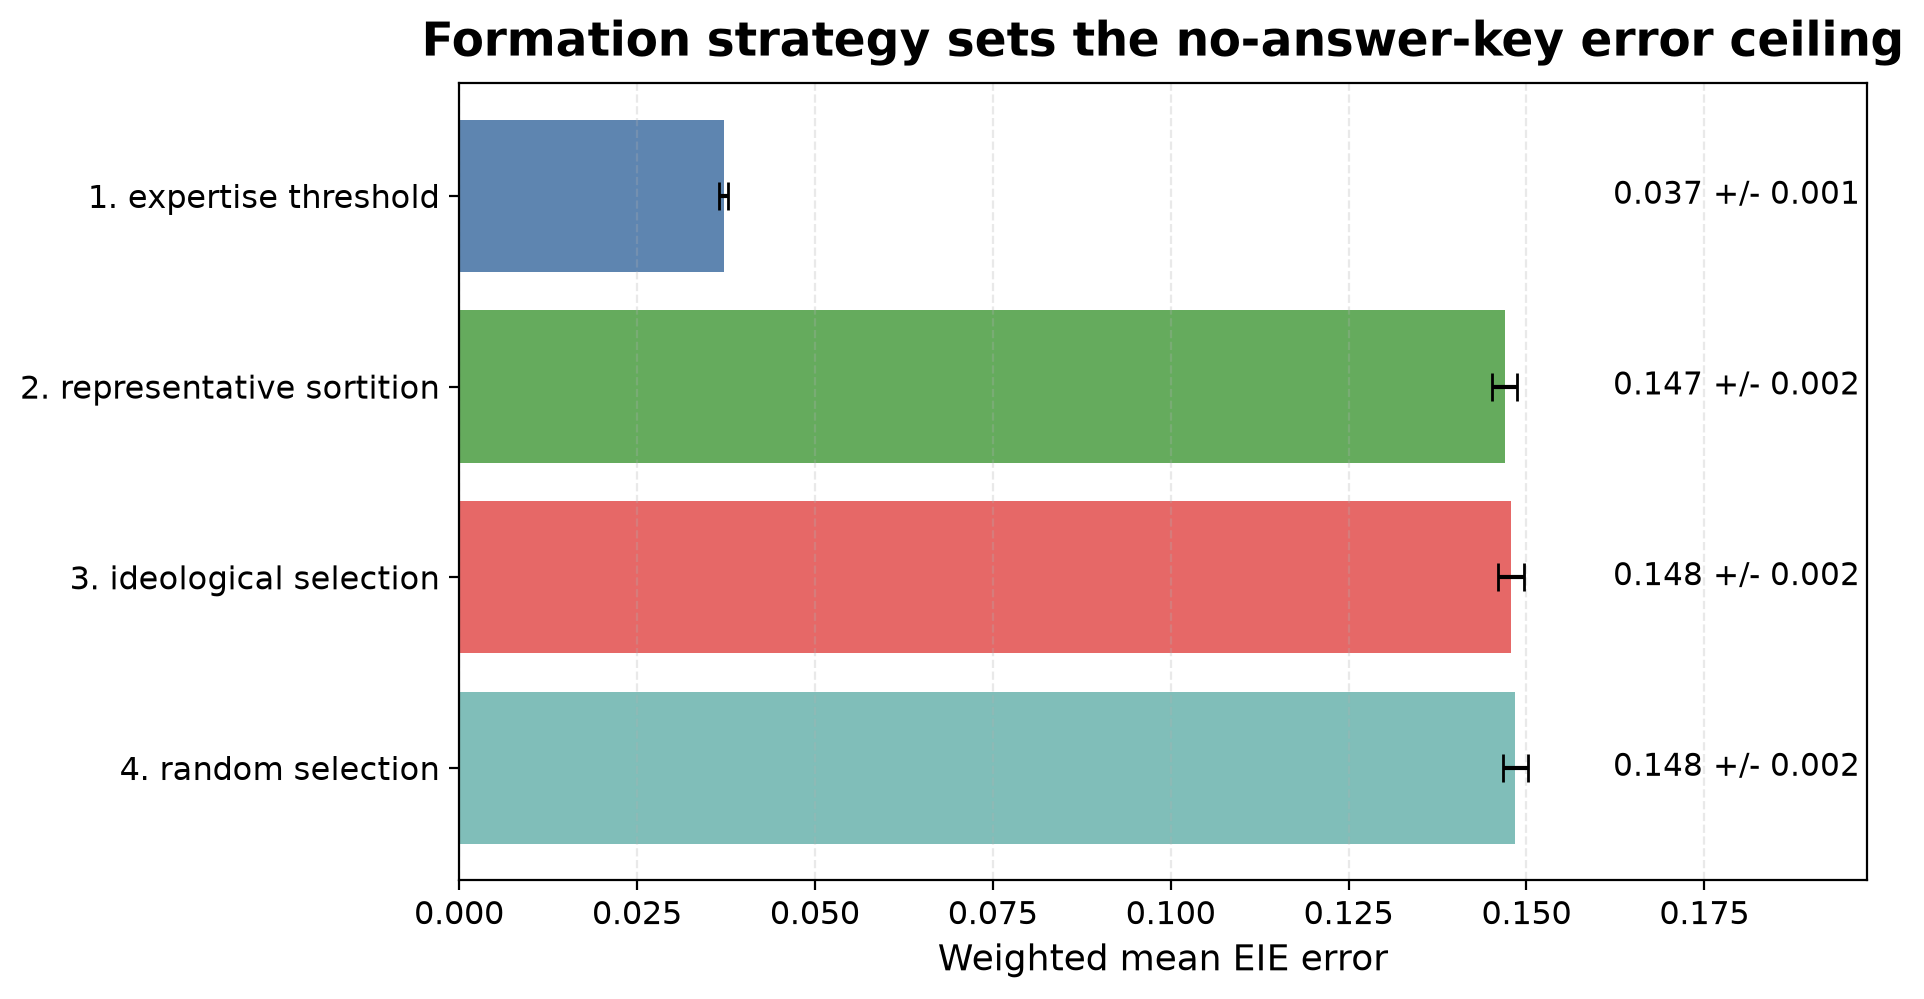
\includegraphics[width=0.75\linewidth,height=0.46\textheight,keepaspectratio,alt={Horizontal bars give the mean oracle-referenced EIE recovery error for each of the four panel-formation strategies, ordered best (lowest, top) to worst (highest, bottom); the whiskers are 95\% confidence intervals over 96 seeds and the value beside each bar is the mean +/- half-interval, all from source output/data/sweep\_aggregated.csv (profile manuscript\_contrast, hash fda4da941cf0). Read it as the ceiling each upstream choice imposes on the downstream blind estimator: competence-first selection sits far left (near-zero error) while the other three strategies cluster together to its right. Claim: the upstream formation rule, not the estimator, sets the no-answer-key error ceiling, and the competence-first-vs-rest gap dwarfs anything the estimator does on a fixed panel; caveat: only the competence-first separation is resolved --- representative, random, and single-bloc selection are statistically indistinguishable from one another, as the power/separation layer certifies.}]{../figures/strategy_ranking.png}
\caption{Horizontal bars give the mean oracle-referenced EIE recovery
error for each of the four panel-formation strategies, ordered best
(lowest, top) to worst (highest, bottom); the whiskers are 95\%
confidence intervals over 96 seeds and the value beside each bar is the
mean +/- half-interval, all from source
\protect\breaktt{output/data/sweep\_aggregated.csv} (profile
manuscript\_contrast, hash fda4da941cf0). Read it as the ceiling each
upstream choice imposes on the downstream blind estimator:
competence-first selection sits far left (near-zero error) while the
other three strategies cluster together to its right. Claim: the
upstream formation rule, not the estimator, sets the no-answer-key error
ceiling, and the competence-first-vs-rest gap dwarfs anything the
estimator does on a fixed panel; caveat: only the competence-first
separation is resolved --- representative, random, and single-bloc
selection are statistically indistinguishable from one another, as the
power/separation layer certifies.}\label{fig:ranking}
\end{figure}

The dominant lever is therefore \emph{whether the panel is curated for
competence at all}, not a graded property of the formation rule. The
competence-first-vs-sortition contrast is a \textbf{resolved} separation
on this instrument: the trio-level bootstrap separation gate reads
\textbf{separated} (means 0.037 vs 0.122), the two strategies' pooled
confidence intervals in the table above are disjoint (0.037 ± 0.003
versus 0.147 ± 0.014), and the power analysis resolves it as
\textbf{significant} (well-powered, not design-limited). Every contrast
\emph{among} the other three is, by contrast, design-indistinguishable
--- including the representative-vs-single-bloc pair, whose effect is
inconclusive (its 95\% CI crosses zero, inconclusive (95\% CI crosses
zero)). So competence-first selection beats the representative draw by a
resolved interval, but representativeness, randomness, and single-bloc
concentration are interchangeable for recovery on this instrument --- a
sharper and more honest result than a four-way ranking would suggest.
\end{block}

\begin{block}{Sortition only separates when the confound rides on the
balanced axis}
\protect\phantomsection\label{sortition-only-separates-when-the-confound-rides-on-the-balanced-axis}
\textbf{H2 (concentrating correlated error degrades recovery).}
\breakseq{[@fig:repideo]} reports the single-bloc-minus-representative EIE
error contrast across the full active regime grid. Positive cells mean
the representative draw has lower post-NTQR recovery error. The axes
expose the design levers directly: expert stringency
(\texttt{mean\_expertise}), ideological bias spread
(\texttt{bias\_std}), and sortition size (\texttt{panel\_size}).

\begin{figure}
\centering
\includegraphics[width=0.92\linewidth,height=0.46\textheight,keepaspectratio,alt={Faceted heatmaps of the single-bloc-minus-representative EIE error contrast across expert stringency (mean expertise, rows), ideological bias spread (columns), and panel size (one facet per size), from source output/data/sweep\_aggregated.csv (profile manuscript\_contrast, hash fda4da941cf0), with analytical sign predictions overlaid from output/data/analytical\_predictions.json. Colour encodes the signed contrast on a diverging scale centred at zero: positive (red) cells mean the representative draw recovers with lower error than the single-bloc draw in that regime, negative (blue) the reverse. Statistic: cell-level mean contrast over 96 seeds; stars mark descriptive 95\% intervals excluding zero. Read across a row to see how stringency modulates the gap and down a column to see the effect of bias concentration. Claim: the representative-vs-single-bloc distinction is not a single number but is regime-dependent, becoming visible only as bias, stringency, and size are jointly varied; caveat: the intervals are descriptive and synthetic-profile bounded, and they are deliberately not pooled with the real Ollama evidence, which lives in the separate Gemma postdoc companion in \breakseq{[@fig:postdocrank]}, \breakseq{[@fig:postdocbias]}, and \breakseq{[@fig:postdocalign]}.}]{../figures/rep_vs_ideo_heatmap.png}
\caption{Faceted heatmaps of the single-bloc-minus-representative EIE
error contrast across expert stringency (mean expertise, rows),
ideological bias spread (columns), and panel size (one facet per size),
from source \protect\breaktt{output/data/sweep\_aggregated.csv} (profile
manuscript\_contrast, hash fda4da941cf0), with analytical sign
predictions overlaid from
\protect\breaktt{output/data/analytical\_predictions.json}. Colour
encodes the signed contrast on a diverging scale centred at zero:
positive (red) cells mean the representative draw recovers with lower
error than the single-bloc draw in that regime, negative (blue) the
reverse. Statistic: cell-level mean contrast over 96 seeds; stars mark
descriptive 95\% intervals excluding zero. Read across a row to see how
stringency modulates the gap and down a column to see the effect of bias
concentration. Claim: the representative-vs-single-bloc distinction is
not a single number but is regime-dependent, becoming visible only as
bias, stringency, and size are jointly varied; caveat: the intervals are
descriptive and synthetic-profile bounded, and they are deliberately not
pooled with the real Ollama evidence, which lives in the separate Gemma
postdoc companion in \breakseq{[@fig:postdocrank]}, \breakseq{[@fig:postdocbias]}, and
\breakseq{[@fig:postdocalign]}.}\label{fig:repideo}
\end{figure}

On this baseline grid the contrast is design-limited and must be read
cell by cell: the analytical prediction is directional (single-bloc
ideological selection should not beat representative sortition when bias
is the manipulated dependence source), and the heatmap shows where the
regenerated synthetic data aligns, where it remains uncertain, and where
the active design is too small to resolve a sign. This grid cannot fan
the strategies apart because it never realizes H2's premise --- its
judges err independently; the composition-coupled confound that supplies
the missing channel, and resolves H2, is reported in
§Composition-coupled correlation fans the strategies apart.
\end{block}

\begin{block}{NTQR beats majority voting only in selected regimes}
\protect\phantomsection\label{ntqr-beats-majority-voting-only-in-selected-regimes}
For the pre/post comparison, ``pre-NTQR'' means the supervised
majority-vote baseline already stored as \texttt{mv\_error};
``post-NTQR'' means the ground-truth-free EIE recovery error stored as
\texttt{eie\_error}. \breakseq{[@fig:prepost]} plots \texttt{EIE\ -\ MV}, so
negative cells mean the NTQR recovery estimate is closer to the
supervised oracle than the majority-vote baseline for that regime.

\begin{figure}
\centering
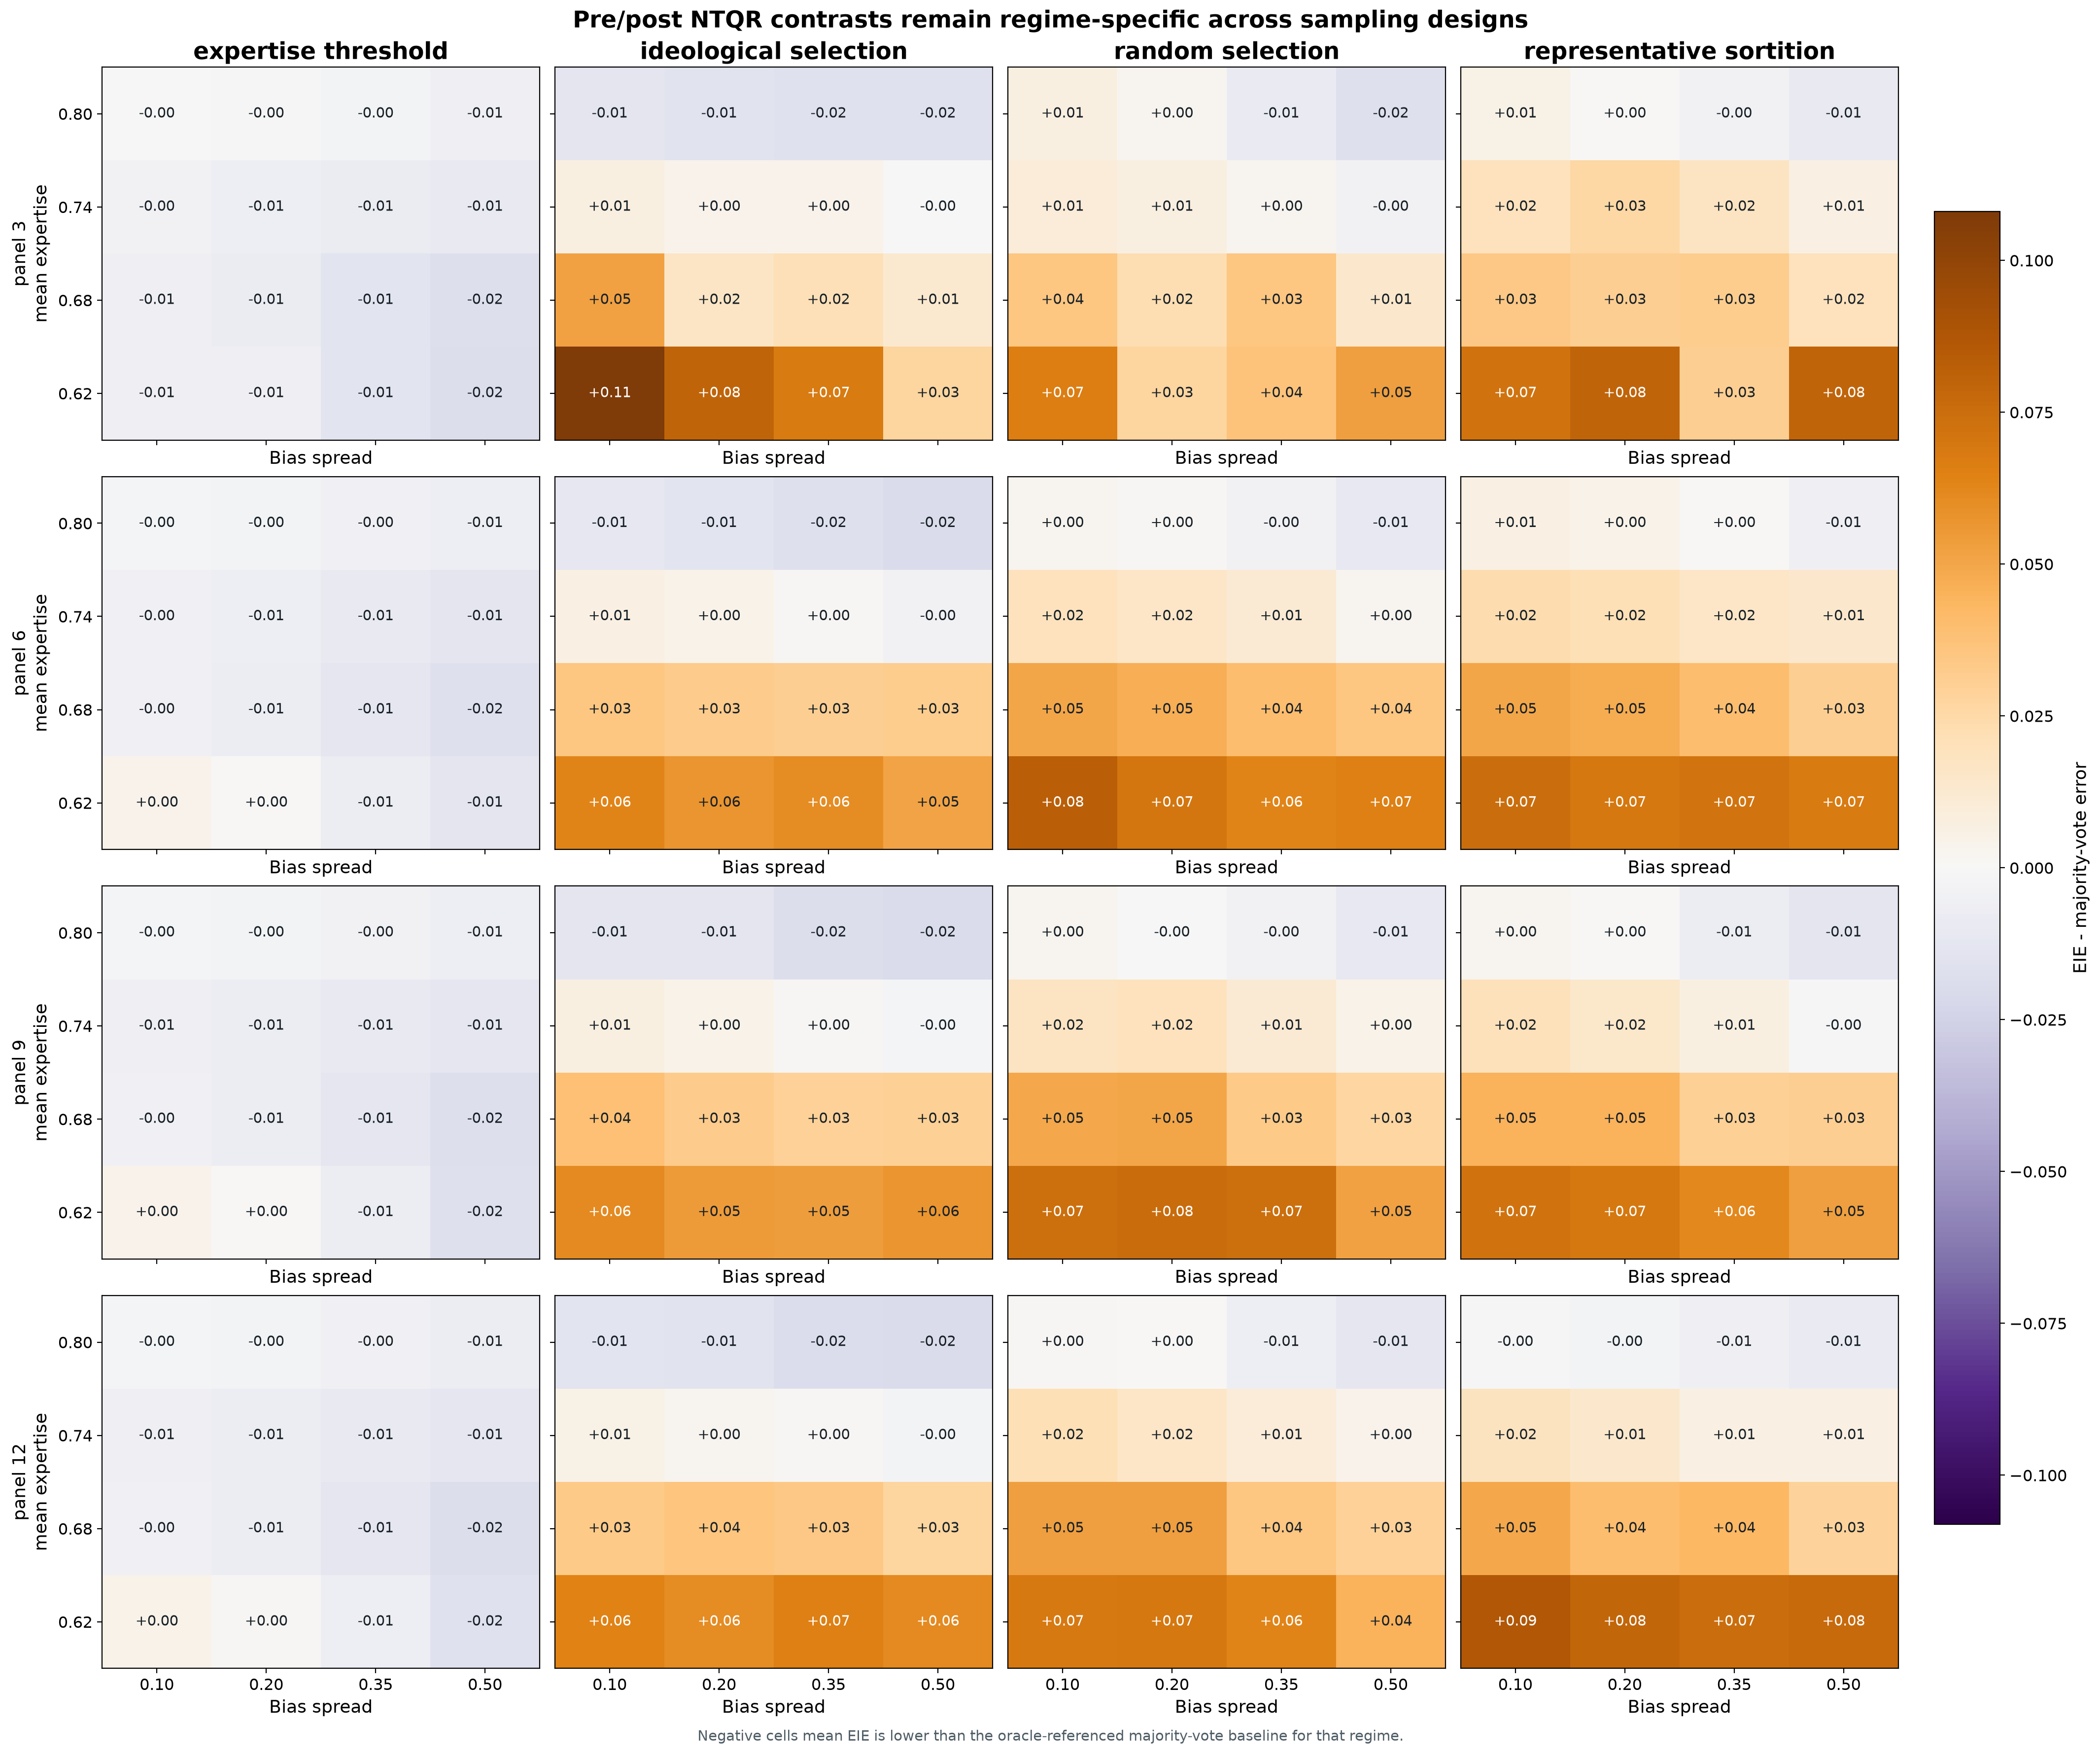
\includegraphics[width=0.95\linewidth,height=0.46\textheight,keepaspectratio,alt={Faceted heatmaps contrasting the post-NTQR error-independent estimate against the pre-NTQR supervised majority-vote baseline, broken out by strategy, panel size, expert stringency, and bias spread, from source output/data/analytical\_predictions.json, derived in turn from output/data/sweep\_aggregated.csv (profile manuscript\_contrast, hash fda4da941cf0). Colour encodes the signed difference on a diverging scale: negative (blue) cells are where the blind NTQR recovery lands closer to the oracle than the majority-vote baseline did, positive (red) where it does not. Statistic: cell-level mean difference over 96 seeds; metric is eie\_mean - mv\_mean, so the figure isolates what the estimator adds (or costs) on top of naive voting. Claim: panel size and bias act on each formation strategy differently before and after NTQR recovery, so there is no uniform pre/post improvement; caveat: this is oracle-referenced simulation on synthetic labels, not a live-judge validation claim.}]{../figures/pre_post_ntqr_heatmap.png}
\caption{Faceted heatmaps contrasting the post-NTQR error-independent
estimate against the pre-NTQR supervised majority-vote baseline, broken
out by strategy, panel size, expert stringency, and bias spread, from
source \protect\breaktt{output/data/analytical\_predictions.json},
derived in turn from \protect\breaktt{output/data/sweep\_aggregated.csv}
(profile manuscript\_contrast, hash fda4da941cf0). Colour encodes the
signed difference on a diverging scale: negative (blue) cells are where
the blind NTQR recovery lands closer to the oracle than the
majority-vote baseline did, positive (red) where it does not. Statistic:
cell-level mean difference over 96 seeds; metric is
\protect\breaktt{eie\_mean\ -\ mv\_mean}, so the figure isolates what the
estimator adds (or costs) on top of naive voting. Claim: panel size and
bias act on each formation strategy differently before and after NTQR
recovery, so there is no uniform pre/post improvement; caveat: this is
oracle-referenced simulation on synthetic labels, not a live-judge
validation claim.}\label{fig:prepost}
\end{figure}

The companion alignment map (\breakseq{[@fig:theoryalign]}) makes the
analytical layer auditable rather than rhetorical. Each cell reports how
many expertise levels in that size-bias slice match the directional
prediction that ideological-minus-representative EIE should be positive.
The same JSON artifact also records the monotone checks for bias and
expertise.

\begin{figure}
\centering
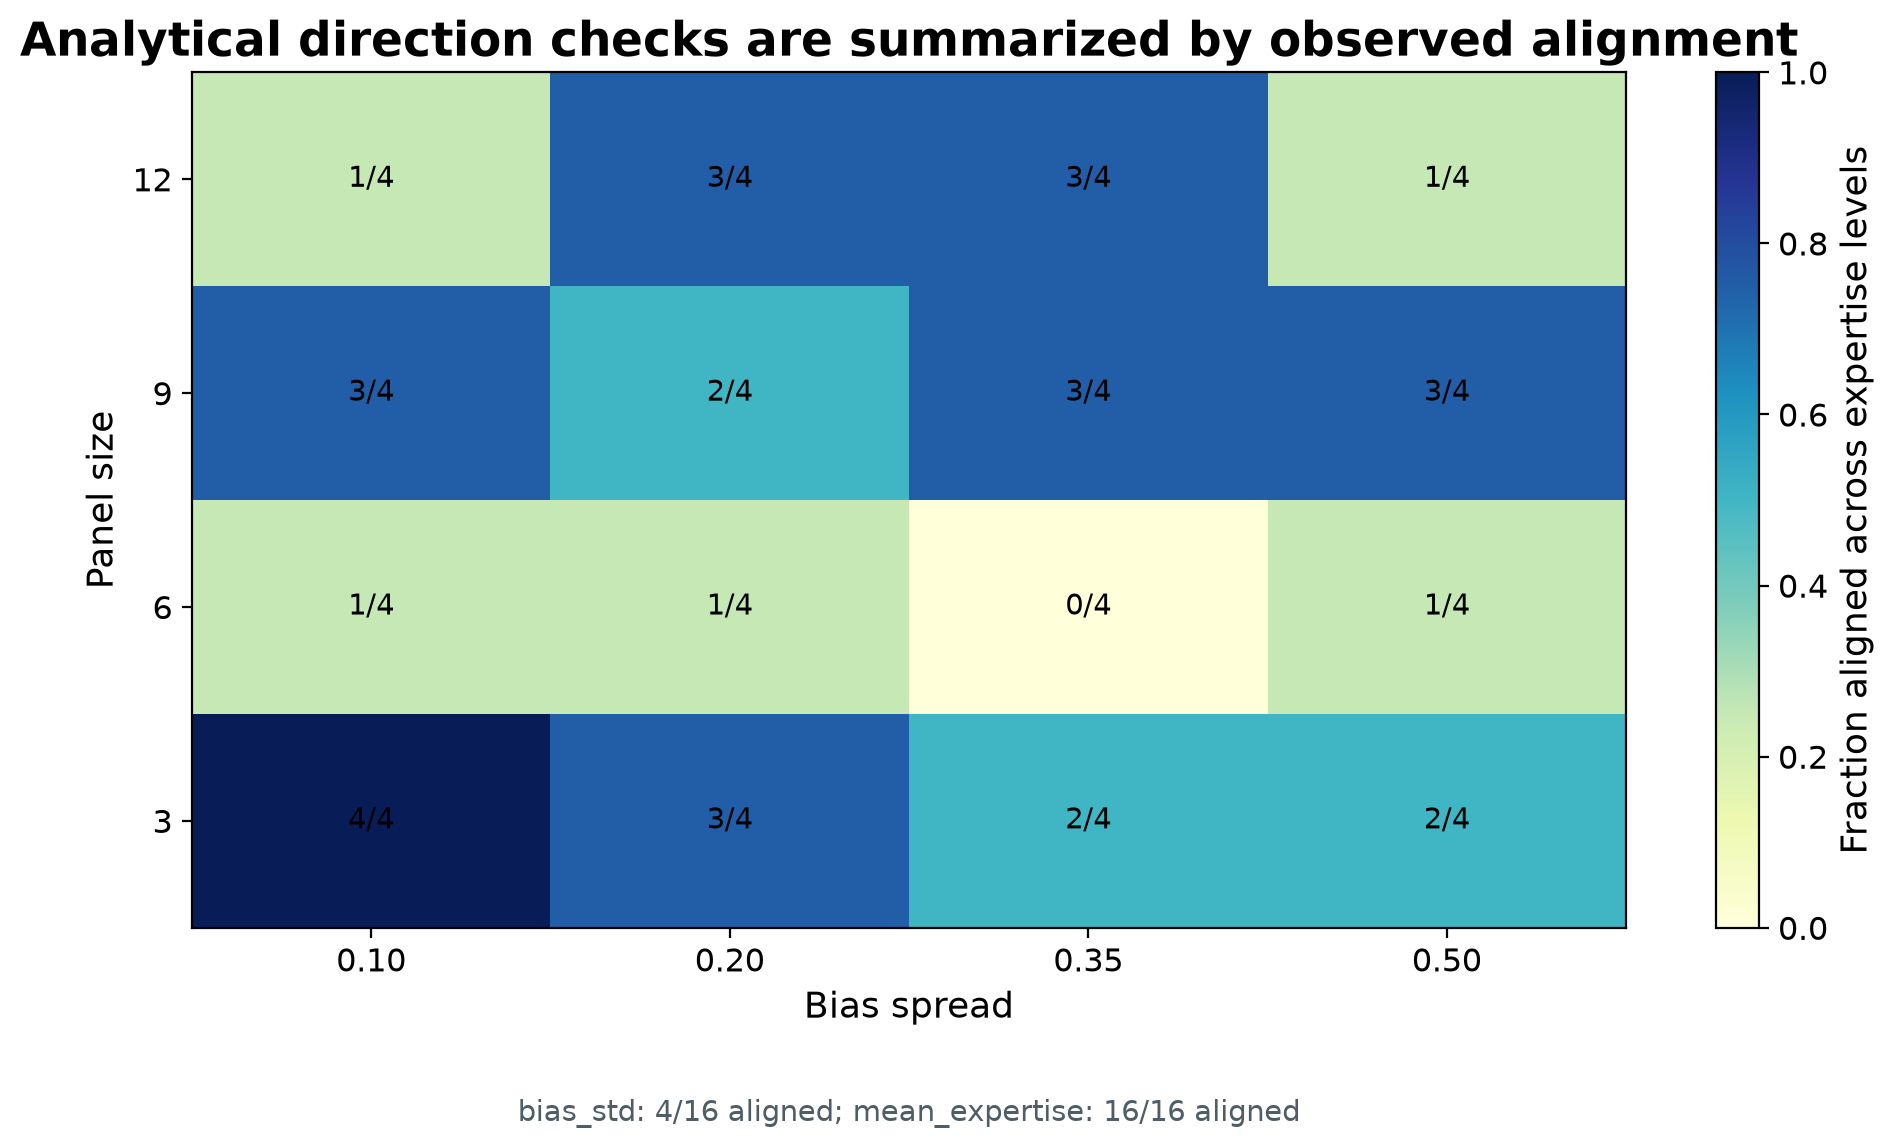
\includegraphics[width=0.72\linewidth,height=0.46\textheight,keepaspectratio,alt={Audit heatmap of how often the analytical directional predictions match the regenerated synthetic cells, from source output/data/analytical\_predictions.json. Each cell of a panel-size x bias-spread slice reports the count of expertise levels whose observed contrast sign agrees with the predicted sign; darker cells mean more of the expertise levels in that slice align with the prediction. Statistic: aligned expertise-level cells per panel-size x bias slice, over source sweep profile manuscript\_contrast, 96 seeds. The figure exists to make the analytical layer falsifiable rather than rhetorical: a prediction that systematically disagreed with the data would show as pale cells. Claim: analytical expectations are checked against regenerated artifacts rather than asserted in prose; caveat: the predictions are directional and order constraints only, not closed-form numerical EIE laws, so partial agreement is expected and is reported honestly.}]{../figures/theory_vs_observed_alignment.png}
\caption{Audit heatmap of how often the analytical directional
predictions match the regenerated synthetic cells, from source
\protect\breaktt{output/data/analytical\_predictions.json}. Each cell of
a panel-size x bias-spread slice reports the count of expertise levels
whose observed contrast sign agrees with the predicted sign; darker
cells mean more of the expertise levels in that slice align with the
prediction. Statistic: aligned expertise-level cells per panel-size x
bias slice, over source sweep profile manuscript\_contrast, 96 seeds.
The figure exists to make the analytical layer falsifiable rather than
rhetorical: a prediction that systematically disagreed with the data
would show as pale cells. Claim: analytical expectations are checked
against regenerated artifacts rather than asserted in prose; caveat: the
predictions are directional and order constraints only, not closed-form
numerical EIE laws, so partial agreement is expected and is reported
honestly.}\label{fig:theoryalign}
\end{figure}
\end{block}

\begin{block}{Larger panels are a neutral sampling knob here}
\protect\phantomsection\label{larger-panels-are-a-neutral-sampling-knob-here}
\textbf{H3 (size is a sampling knob, not a uniform improvement).}
\breakseq{[@fig:powercurve]} plots EIE error against panel/ensemble size for
each strategy. If size were a clean power knob, every curve would fall
from size 3 to size 6. It does not:

{\def\LTcaptype{none} % do not increment counter
\begin{longtable}[]{@{}llll@{}}
\toprule\noalign{}
Strategy & Size 3 & Size 6 & Pooled direction \\
\midrule\noalign{}
\endhead
expertise threshold & 0.037 & 0.038 & roughly flat \\
representative sortition & 0.122 & 0.154 & error rises \\
random selection & 0.118 & 0.155 & error rises \\
ideological selection & 0.124 & 0.151 & error rises \\
\bottomrule\noalign{}
\end{longtable}
}

\begin{figure}
\centering
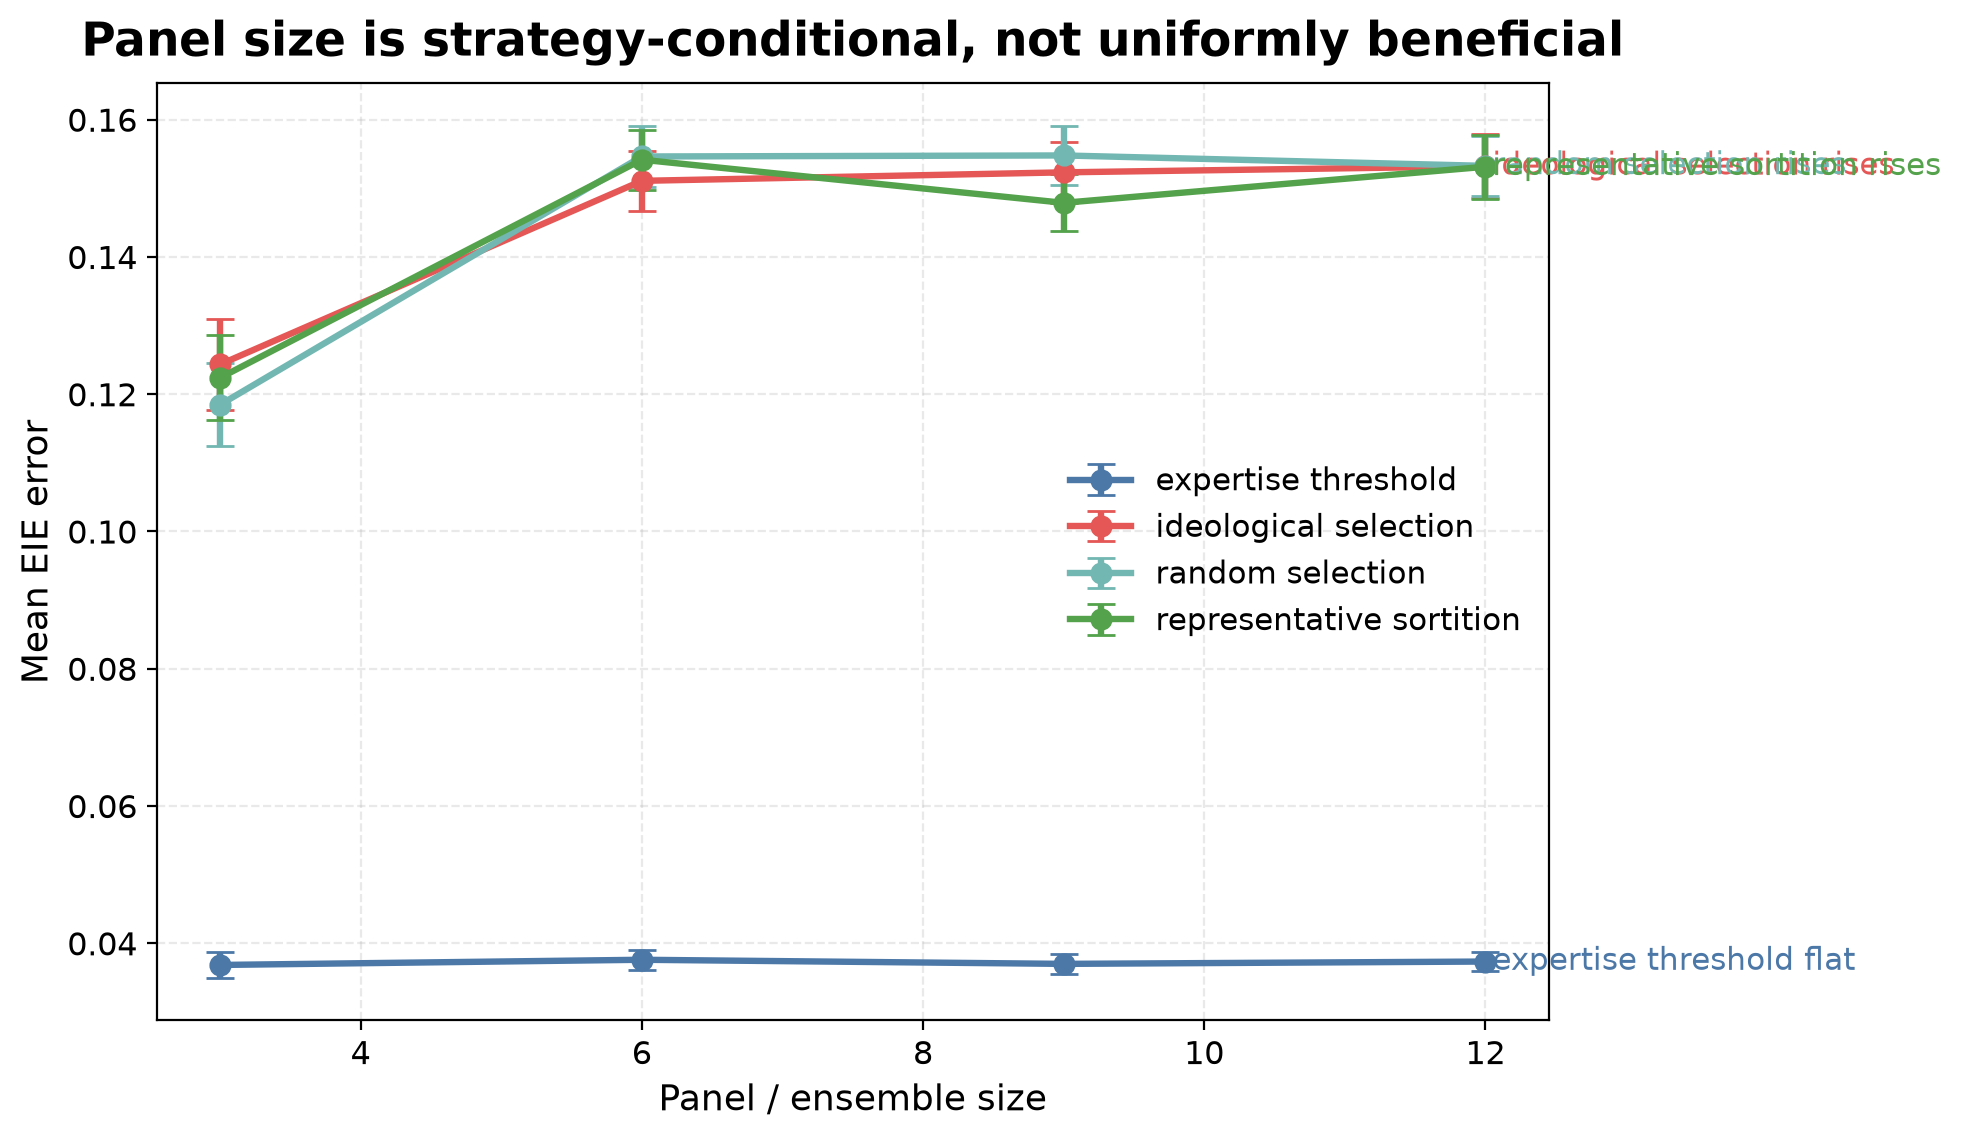
\includegraphics[width=0.75\linewidth,height=0.46\textheight,keepaspectratio,alt={One line per panel-formation strategy tracing mean EIE recovery error against panel/ensemble size (3, 6, 9, 12 members), from source output/data/sweep\_results.json, aggregated over 96 seeds with per-point 95\% confidence intervals and a colour-matched end-label summarising each curve's trio-to-six-seat direction. If size were a clean power knob every curve would fall monotonically left to right; instead the curves cross. Read the vertical spread at any size as the strategy gap and each curve's slope as the strategy-specific effect of adding experts. Claim: a paired regime-controlled test (paired\_size\_contrast) resolves a trio-to-six-seat size effect for three of the four strategies, but every resolved increase is tiny and single-bloc is within noise, so size is essentially neutral at this grid and the dominant lever is which strategy forms the panel; caveat: this pooled curve marginalizes over sixteen regimes and is bounded to the active sweep profile.}]{../figures/power_curve.png}
\caption{One line per panel-formation strategy tracing mean EIE recovery
error against panel/ensemble size (3, 6, 9, 12 members), from source
\protect\breaktt{output/data/sweep\_results.json}, aggregated over 96
seeds with per-point 95\% confidence intervals and a colour-matched
end-label summarising each curve's trio-to-six-seat direction. If size
were a clean power knob every curve would fall monotonically left to
right; instead the curves cross. Read the vertical spread at any size as
the strategy gap and each curve's slope as the strategy-specific effect
of adding experts. Claim: a paired regime-controlled test
(\protect\breaktt{paired\_size\_contrast}) resolves a trio-to-six-seat
size effect for three of the four strategies, but every resolved
increase is tiny and single-bloc is within noise, so size is essentially
neutral at this grid and the dominant lever is which strategy forms the
panel; caveat: this pooled curve marginalizes over sixteen regimes and
is bounded to the active sweep profile.}\label{fig:powercurve}
\end{figure}

Those Size-3/Size-6 cells and the figure's end-labels are \textbf{pooled
point estimates} over sixteen regimes. The powered test is a
\textbf{paired} contrast that matches each regime-and-seed cell across
the two sizes (\breaktt{paired\_size\_contrast} in
\breaktt{src/ntqr\_allotment/power\_study.py}), removing the
between-regime variance. Under that test 3 of the four strategies show a
\emph{resolved} trio-to-six-seat change, and every resolved change is a
small \textbf{increase} in error: random selection (+0.015, 95\% CI
{[}+0.009, +0.021{]}), representative sortition (+0.007, CI {[}+0.001,
+0.012{]}), and competence-first selection (+0.004, CI {[}+0.003,
+0.005{]}); only single-bloc selection (-0.003, CI {[}-0.007, +0.002{]})
is within noise. These effects are \textbf{resolved but negligible} ---
the largest, +0.015, is about a tenth of the bottom-tier baseline near
0.148. So more experts do not help, and at most very slightly hurt: we
reject the simple hypothesis that more experts always help, but the
honest reading is that \textbf{size is essentially neutral} at this
grid, and the dominant lever is \textbf{strategy}, not size.

\textbf{What the size diagnostic rules out.} The error-independent
solver assumes the three judges' errors are uncorrelated, so the natural
guess is that larger panels feed the ensemble more error-correlated
trios. A per-trio diagnostic refutes that guess (\breakseq{[@fig:triocond]},
\breaktt{src/ntqr\_allotment/trio\_conditioning.py}, over 17,126 usable
trios). The realized mean absolute pairwise error-correlation --- the
quantity the solver assumes is zero --- is \textbf{essentially flat}
across the size ladder for every strategy (0.0087 at the trio to 0.0101
at twelve seats), so enlarging the panel does not feed the ensemble more
correlated trios. Correlation \emph{is} a relevant axis --- within a
strategy, higher-correlation trios recover worse (Pearson up to +0.70
for competence-first) --- but because correlation does not grow with
size, it does not identify a positive mechanism for the tiny paired size
deltas. No single per-trio summary statistic (correlation, judge
accuracy, or scan position) predicts the per-trio error strongly enough
to pin the remaining cost on worse judges. We therefore report the small
paired size deltas after ruling out the main correlation explanation,
not as an affirmative aggregation effect.

\begin{figure}
\centering
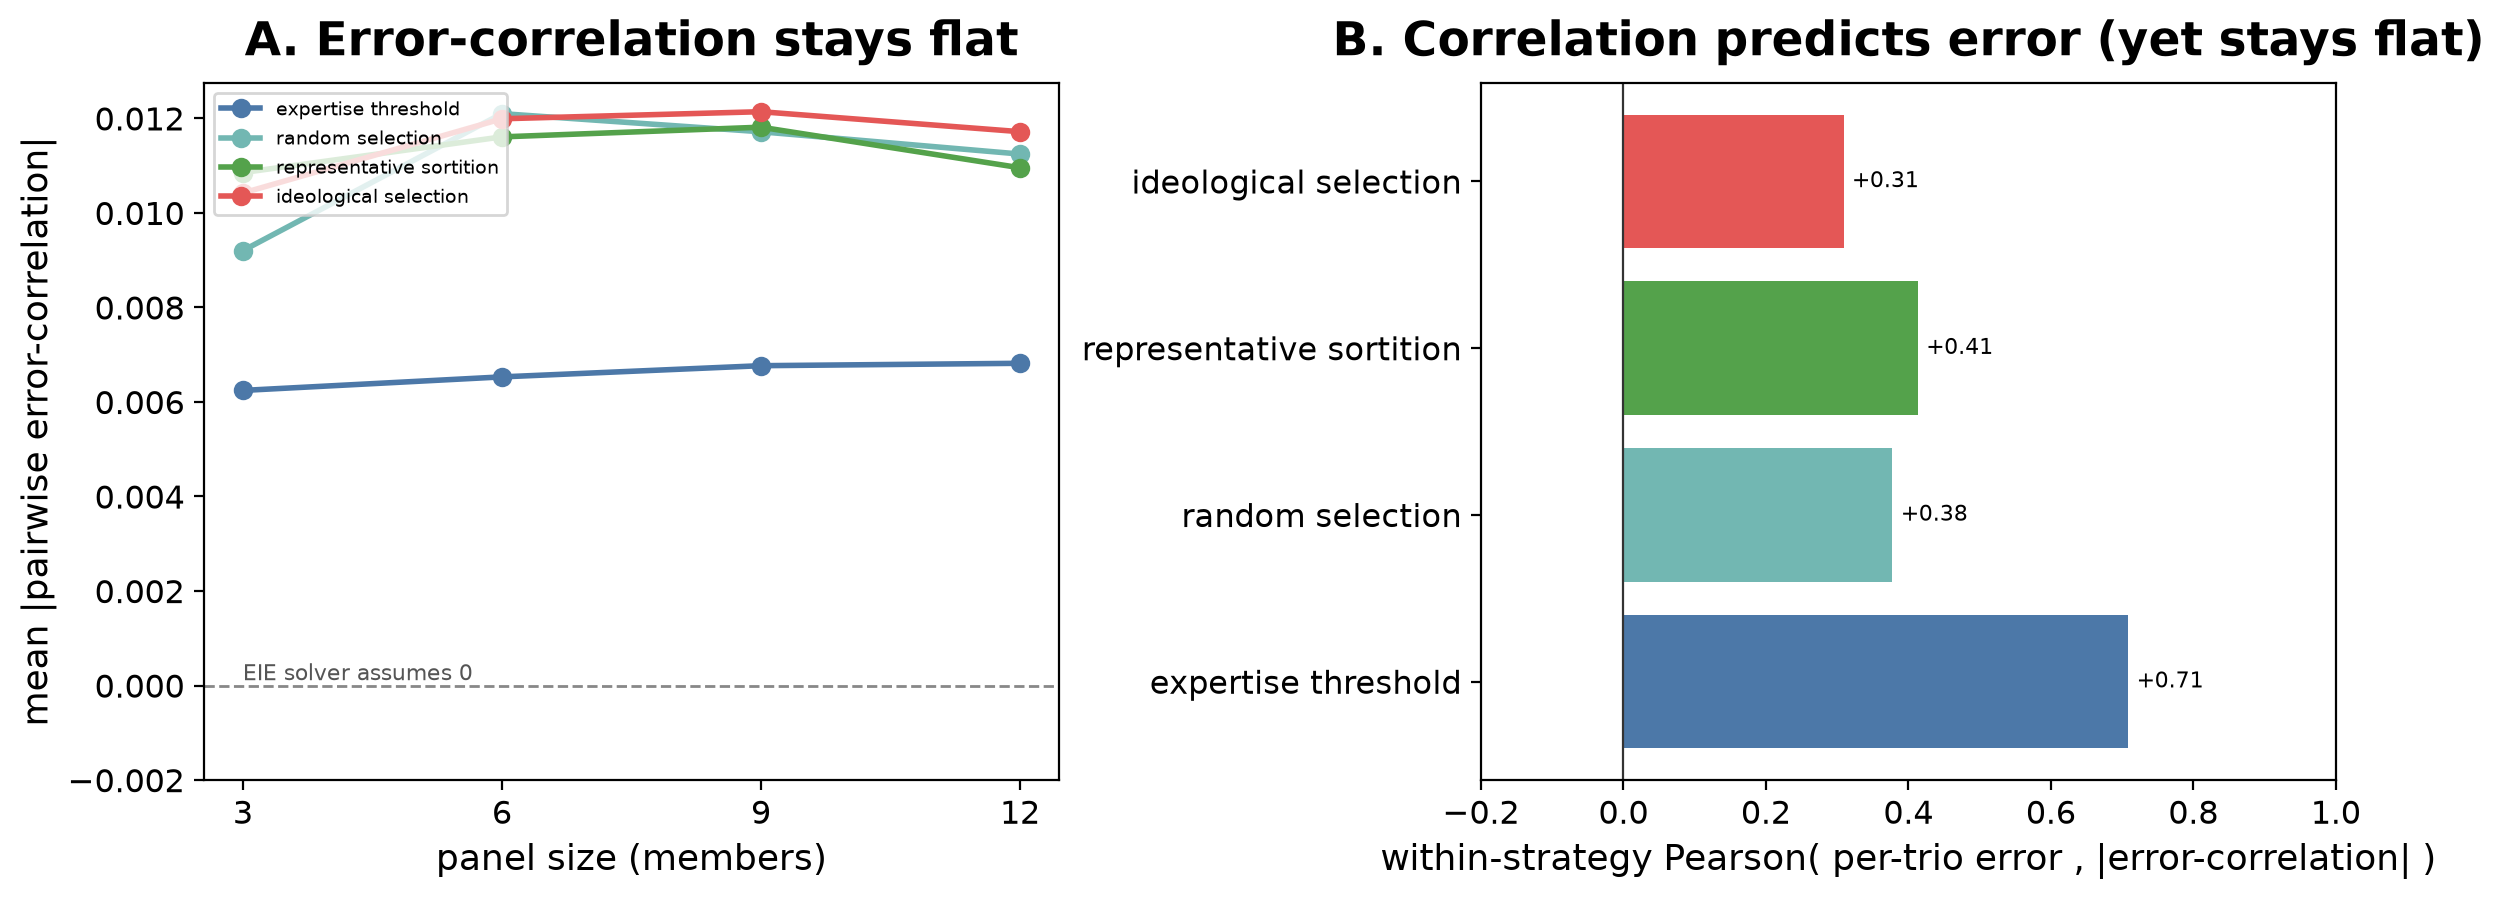
\includegraphics[width=0.9\linewidth,height=0.46\textheight,keepaspectratio,alt={Two-panel per-trio mechanism diagnostic for the panel-size contrast, from source output/data/trio\_conditioning.json (17,126 usable trios over 12 seeds of the reported regime grid). Panel A plots the mean absolute pairwise error-correlation of the usable trios against panel size, one line per formation strategy, with a dashed reference at zero (the value the error-independent solver assumes); every line holds the small 0.0087-to-0.0105 baseline rather than rising, so enlarging the panel does not pull in more error-correlated trios. Panel B plots the within-strategy Pearson correlation between a trio's recovery error and its absolute error-correlation; the bars are positive (up to +0.70 for competence-first), so correlation genuinely predicts per-trio error --- it simply does not grow with size. Statistic: mean absolute error-correlation by size (A) and within-strategy Pearson of per-trio error against absolute error-correlation (B), measured over the same usable trios the ensemble-of-trios averages. Claim: the diagnostic rules out a size-growing error-correlation mechanism; caveat: it does not identify a positive mechanism and remains a 12-seed structural diagnostic on synthetic labels, not a headline confidence interval.}]{../figures/trio_conditioning.png}
\caption{Two-panel per-trio mechanism diagnostic for the panel-size
contrast, from source
\protect\breaktt{output/data/trio\_conditioning.json} (17,126 usable
trios over 12 seeds of the reported regime grid). Panel A plots the mean
absolute pairwise error-correlation of the usable trios against panel
size, one line per formation strategy, with a dashed reference at zero
(the value the error-independent solver assumes); every line holds the
small 0.0087-to-0.0105 baseline rather than rising, so enlarging the
panel does not pull in more error-correlated trios. Panel B plots the
within-strategy Pearson correlation between a trio's recovery error and
its absolute error-correlation; the bars are positive (up to +0.70 for
competence-first), so correlation genuinely predicts per-trio error ---
it simply does not grow with size. Statistic: mean absolute
error-correlation by size (A) and within-strategy Pearson of per-trio
error against absolute error-correlation (B), measured over the same
usable trios the ensemble-of-trios averages. Claim: the diagnostic rules
out a size-growing error-correlation mechanism; caveat: it does not
identify a positive mechanism and remains a 12-seed structural
diagnostic on synthetic labels, not a headline confidence
interval.}\label{fig:triocond}
\end{figure}
\end{block}

\begin{block}{Global injected correlation is measurable but
recovery-limited}
\protect\phantomsection\label{global-injected-correlation-is-measurable-but-recovery-limited}
\textbf{H4 (error-correlation is measurable; recovery should degrade
with it).} The centerpiece measurement injects a controlled
error-correlation \(\rho\) into a trio's votes, measures the
\emph{realized} correlation NTQR itself reports
(\texttt{mean\_abs\_pair}), computes the unlabeled EIE evaluation, and
scores it against the supervised oracle
(\breaktt{output/data/independence\_sweep.csv}, produced by
\breaktt{src/ntqr\_allotment/independence\_sweep.py}). The robust,
monotone finding is that \textbf{the realized correlation rises with the
injected \(\rho\)}: averaged over the non-degenerate cells it climbs
from 0.019 at the lowest injected \(\rho\) to 0.123 at the highest. The
injection knob does what it claims --- it manufactures measurable
error-correlation, and NTQR's own correlation diagnostic registers it.

\begin{figure}
\centering
\includegraphics[width=0.75\linewidth,height=0.46\textheight,keepaspectratio,alt={Oracle-referenced EIE error (y-axis) versus the realized pairwise error correlation \textbackslash rho\_\{\textbackslash mathrm\{NTQR\}\} that the NTQR estimator itself measures from the votes (x-axis), shown as a scatter with one point per non-degenerate (\textbackslash rho, strategy) cell of the tolerance sweep, from source output/data/independence\_sweep.csv. The x-axis is the quantity the exact solver assumes is zero; the controlled injection knob moves points rightward, which verifies the diagnostic, while the y-axis tests whether more correlation actually costs recovery accuracy. Claim: injected \textbackslash rho creates measurable NTQR error correlation (points do move right), but the fitted recovery-error trend is unresolved at this grid; statistic: OLS error-vs-correlation slope -0.145 with 95\% bootstrap CI {[}-4.335, 0.911{]}, which crosses zero; caveat: this figure supports the correlation diagnostic only, not a resolved recovery-effect law.}]{../figures/error_vs_correlation.png}
\caption{Oracle-referenced EIE error (y-axis) versus the realized
pairwise error correlation \(\rho_{\mathrm{NTQR}}\) that the NTQR
estimator itself measures from the votes (x-axis), shown as a scatter
with one point per non-degenerate (\(\rho\), strategy) cell of the
tolerance sweep, from source
\protect\breaktt{output/data/independence\_sweep.csv}. The x-axis is the
quantity the exact solver assumes is zero; the controlled injection knob
moves points rightward, which verifies the diagnostic, while the y-axis
tests whether more correlation actually costs recovery accuracy. Claim:
injected \(\rho\) creates measurable NTQR error correlation (points do
move right), but the fitted recovery-error trend is unresolved at this
grid; statistic: OLS error-vs-correlation slope -0.145 with 95\%
bootstrap CI {[}-4.335, 0.911{]}, which crosses zero; caveat: this
figure supports the correlation diagnostic only, not a resolved
recovery-effect law.}\label{fig:tolerance}
\end{figure}

Recovery error against the oracle, by contrast, shows \textbf{no
detectable monotone relationship} with that correlation on this grid.
The sweep fixes the panel at the trio (the exact solver's unit) and
varies only \(\rho\) and strategy over up to six seeds per cell, so each
(\(\rho\), strategy) contributes one independent cell to the regression
--- no size-invariant duplicate trio is double-counted. The
ordinary-least-squares slope of recovery error on realized correlation
across those unique cells is -0.145, but its 95\% bootstrap confidence
interval is {[}-4.335, 0.911{]} --- it \textbf{crosses zero}. The honest
verdict is therefore that the fitted slope is \textbf{statistically
indistinguishable from zero} at this 24-expert / 120-item grid.
Crucially this is an \emph{unresolved} result, not evidence of \emph{no}
effect: a CI that spans zero is consistent with a small positive slope,
a small negative one, or none, and this grid is simply too small to
choose between them (mean EIE error 0.367 at the lowest injected
\texttt{rho} and 0.228 at the highest, with a non-monotone dip in
between). We report the interval rather than a bare point estimate
precisely because a single noisy slope on eight cells would overclaim a
precision the data do not support.

What the instrument \emph{does} establish here is narrower and robust:
the realized correlation tracks the injected correlation (the monotone
rise above). The \emph{analytical} expectation encoded in
\texttt{theory.py} (\breaktt{predicted\_error\_vs\_correlation}) is that
recovery error should \textbf{not decrease} as positive
error-correlation grows, because correlation violates the
error-independence the exact solver assumes. That expectation is
\textbf{not confirmed on this global-injection grid}:
\breaktt{independence\_sweep.csv} shows a slight, non-monotone
\emph{decrease} (0.367 at the lowest injected \texttt{rho} to 0.228 at
the highest, slope 95\% CI crossing zero). We now attribute that
non-monotonicity to a \textbf{disclosed limitation of this particular
injection model}, not to small-grid noise alone:
\breaktt{dependence.sample\_votes\_correlated} mixes a shared and an
independent \emph{uniform} latent, and a convex combination of uniforms
is not uniform, so the model's realized per-judge accuracy is
\textbf{not preserved as \texttt{rho} varies} --- it inflates and then
deflates, peaking near \texttt{rho=0.5}. That accuracy confound moves
recovery error in its own right and contaminates the
recovery-vs-correlation slope. Rather than re-engineer this diagnostic
(which would perturb a shipped result), we draw the H4 recovery
conclusion from the \textbf{marginal-accuracy-preserving
composition-coupled instrument} of the following subsection
(§Composition-coupled correlation fans the strategies apart), which
holds each judge's accuracy fixed by construction and resolves the
recovery-vs-correlation relationship in the affirmative
(\breakseq{[@fig:blocphase]}). The global-injection sweep remains in the paper
as the correlation \emph{diagnostic} (the realized correlation does rise
with \texttt{rho}) with its accuracy artifact disclosed. This is a
\textbf{measured behaviour under controlled correlation}, validated in
simulation only; it does \emph{not} show that sortition restores low
oracle-referenced error on real prompted judges. The live Gemma
postdoctoral-review panel that probes the same sampling mechanism on a
local LLM is reported in the Real-Ollama results subsection.
\end{block}

\begin{block}{Composition-coupled correlation exposes the sortition
mechanism}
\protect\phantomsection\label{composition-coupled-correlation-exposes-the-sortition-mechanism}
The H4 slope above is unresolved for a specific, fixable reason. The
tolerance sweep injects a \emph{global} correlation onto a \emph{fixed}
trio, identically for every strategy, so it measures sensitivity to
correlation \textbf{decoupled from how the panel was formed}. That is
the wrong instrument for H2, whose premise is that single-bloc selection
\emph{seats judges whose errors are correlated} --- a premise the
baseline generator never realizes, because there ideology shifts only
each judge's \emph{marginal} accuracy and every judge errs from an
independent stream. Under that generator representative, random, and
single-bloc panels are indistinguishable not by coincidence but
\textbf{by construction}: the channel that would separate them does not
exist, so no parameter sweep over the baseline can fan them out.

We close that gap with a composition-coupled confound
(\breaktt{src/ntqr\_allotment/bloc\_confound.py}). Judges who share an
ideological bloc draw a shared latent \emph{error shock} through a
Gaussian copula of within-group strength \(\rho\); the construction
preserves each judge's per-label accuracy exactly, so any change in
recovery is attributable to error \emph{correlation}, not to an accuracy
shift, and \(\rho=0\) reproduces the independent baseline. (The shared
channel is a symmetric competence shock, not directional bias. \(\rho\)
is the latent within-group correlation; what we plot as ``realized
correlation'' is NTQR's own label-conditional error-correlation
statistic, which is much smaller in magnitude than \(\rho\) --- we
report the quantity the solver assumes is zero, never the latent
\(\rho\).) We sweep \(\rho\) across 7 levels, aggregating on average 239
non-degenerate trials per (strategy, \(\rho\)) point over bias-spread,
stringency, panel-size, and seed regimes (\breakseq{[@fig:blocphase]}).

The result is a clean, graded fan-out. At \(\rho=0\) the three
composition strategies collapse exactly as the baseline reported --- the
ideological-minus-representative gap is 0.000. As coupling rises they
fan out: representative sortition stays essentially flat (0.156 to 0.155
EIE error), random selection degrades (0.157 to 0.190), and single-bloc
ideological selection degrades most (0.156 to 0.267), widening the gap
to 0.112 at \(\rho=0.90\). NTQR's own correlation diagnostic makes the
mechanism legible: at high coupling a representative trio carries
measured error-correlation 0.018 while a single-bloc trio carries 0.129
--- bloc-balancing \emph{decorrelates} the shared shock that
bloc-concentration \emph{concentrates}. This resolves \textbf{H2}
(concentrating correlated error does degrade recovery, once the
correlation is composition-coupled) and answers the open \textbf{H4}
recovery slope in the affirmative under a correctly specified,
marginal-preserving instrument. It is not a pooling artifact: in a
paired per-regime test at \(\rho=0.90\), single-bloc error exceeds
representative error in 180/205 matched regimes (paired mean 0.102, 95\%
CI ±0.012). Nor is the averaged subsample cherry-picked by the
degenerate-trio skip: at high coupling the single-bloc panels have the
\emph{lowest} degenerate-trio rate of the four strategies (tracked per
strategy in \breaktt{bloc\_phase\_summary.json}), so dropping ill-posed
trios cannot be what manufactures their degradation --- if anything it
makes the reported gap conservative.

This robustness is \textbf{conditional, not magical}, and a negative
control says so. The protection appears because representative sortition
balances the very axis --- ideology --- that the confound rides on. When
the shared shock is re-keyed to an orthogonal axis the lottery does
\emph{not} balance (expertise tier), representative sortition loses its
immunity: its error climbs from 0.147 to 0.229, and the large
ideological-minus-representative gap of the matched axis (0.112 at
\(\rho=0.90\)) nearly closes under the orthogonal one (0.026). The point
is not that some \emph{other} strategy inherits the protection ---
competence-first selection draws the top experts, who span expertise
tiers, so it does not maximally concentrate the tier axis either --- but
that representativeness on ideology stops mattering once the confound no
longer rides on ideology. The defensible claim is therefore precise:
\textbf{balancing a panel on the axis a shared error rides on preserves
no-answer-key recovery; balancing the wrong axis does not.} That is a
statement about sortition design in simulation, not a blanket
endorsement of representative panels.

\begin{figure}
\centering
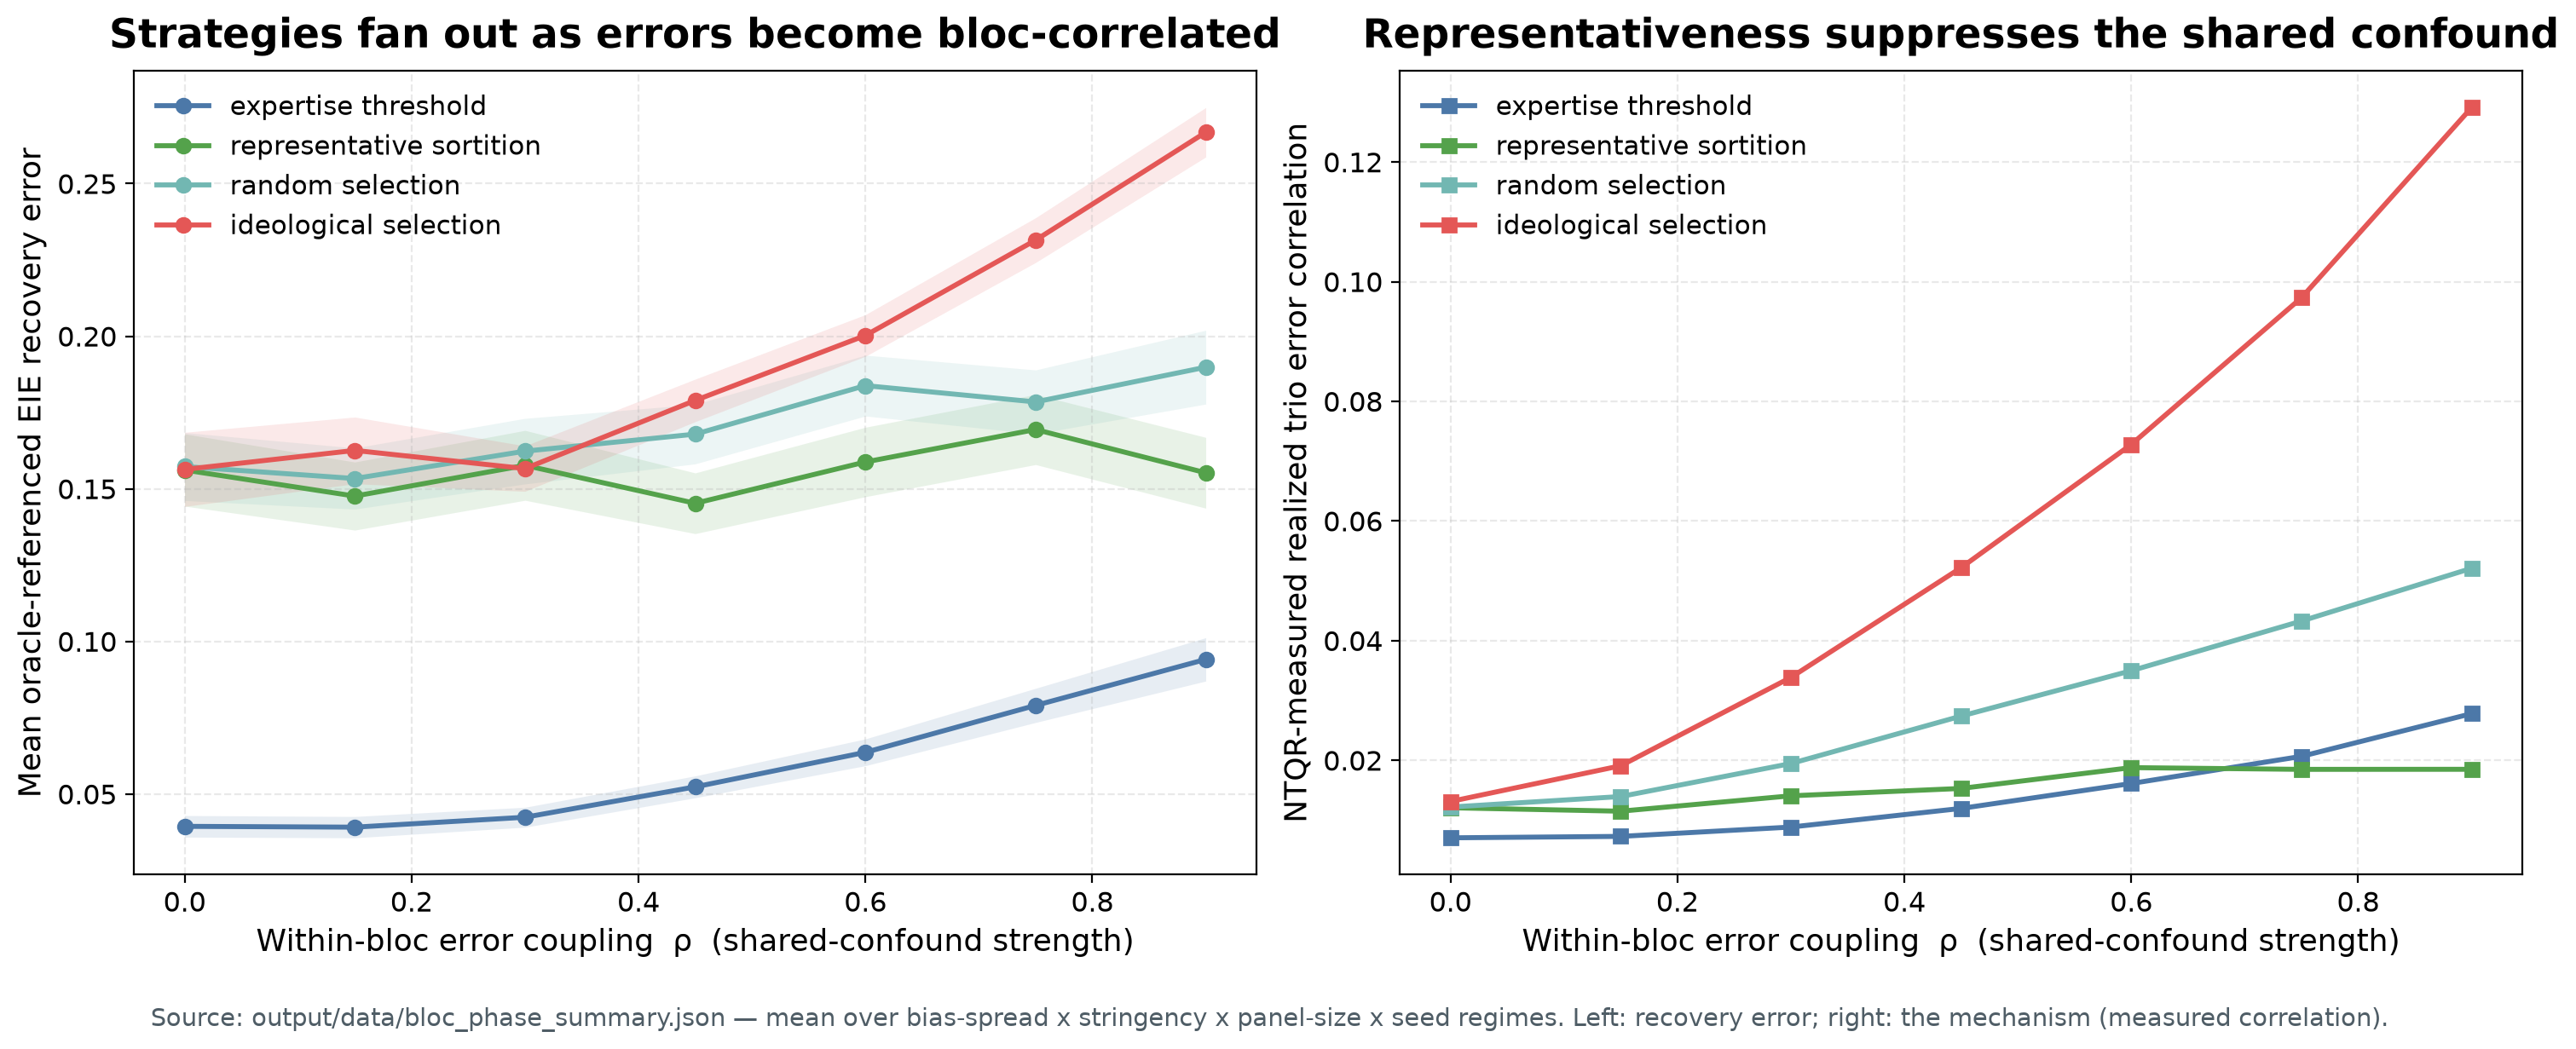
\includegraphics[width=0.95\linewidth,height=0.46\textheight,keepaspectratio,alt={Two-panel bloc-confound phase diagram from source output/data/bloc\_phase\_summary.json, aggregated over bias-spread, stringency, panel-size, and seed regimes. Left: mean oracle-referenced EIE recovery error (y) versus within-bloc error coupling \textbackslash rho (x), one line per panel-formation strategy with 95\% CI bands; the lines coincide at \textbackslash rho=0 (the reproduced baseline collapse) and fan out as \textbackslash rho rises, representative sortition staying flat while single-bloc ideological selection climbs. Right: the NTQR-measured realized trio error correlation (y) versus \textbackslash rho --- the mechanism --- showing representative sortition suppressing the shared confound (flat, low) while single-bloc selection concentrates it (steeply rising). Claim: composition-coupled error correlation makes panel-formation rule the dominant lever on recovery, with representativeness protective specifically when the panel balances the axis the confound rides on; caveat: synthetic, marginal-preserving simulation against a known oracle, and the protection is axis-conditional as the expertise-tier negative control demonstrates.}]{../figures/bloc_phase_diagram.png}
\caption{Two-panel bloc-confound phase diagram from source
\protect\breaktt{output/data/bloc\_phase\_summary.json}, aggregated over
bias-spread, stringency, panel-size, and seed regimes. Left: mean
oracle-referenced EIE recovery error (y) versus within-bloc error
coupling \(\rho\) (x), one line per panel-formation strategy with 95\%
CI bands; the lines coincide at \(\rho=0\) (the reproduced baseline
collapse) and fan out as \(\rho\) rises, representative sortition
staying flat while single-bloc ideological selection climbs. Right: the
NTQR-measured realized trio error correlation (y) versus \(\rho\) ---
the mechanism --- showing representative sortition suppressing the
shared confound (flat, low) while single-bloc selection concentrates it
(steeply rising). Claim: composition-coupled error correlation makes
panel-formation rule the dominant lever on recovery, with
representativeness protective specifically when the panel balances the
axis the confound rides on; caveat: synthetic, marginal-preserving
simulation against a known oracle, and the protection is
axis-conditional as the expertise-tier negative control
demonstrates.}\label{fig:blocphase}
\end{figure}

Representativeness is not only a four-way contrast but a
\textbf{continuous dial}. Fixing the coupling at \(\rho=0.90\) and
forming panels with a tunable single-bloc concentration \(c\) --- from
balanced (\(c=0\), Herfindahl index \(1/B\)) to single-bloc (\(c=1\),
Herfindahl index \(1\)) --- recovery error climbs monotonically from
0.175 to 0.263 across the 6 dial levels (fraction of steps that increase
error: 1.000; \breakseq{[@fig:dial]}). This is the closed-form Herfindahl
account of §Methods made visible: the panel's concentration index over
the confound axis, a closed-form combinatorial statistic, sets its
shared-confound exposure and hence its no-answer-key recovery error.

\begin{figure}
\centering
\includegraphics[width=0.7\linewidth,height=0.46\textheight,keepaspectratio,alt={Single-panel concentration-dial figure from source output/data/bloc\_phase\_summary.json (concentration block), aggregated over bias-spread, stringency, and seed regimes at fixed within-bloc coupling. The x-axis is the single-bloc concentration dial c (the panel's Herfindahl index runs 1/B at c=0 to 1 at c=1). Left y-axis (circles, with 95\% CI band): mean oracle-referenced EIE recovery error; right y-axis (squares): the NTQR-measured realized trio error correlation. Recovery error rises monotonically with concentration, while the realized correlation rises and then saturates once the scored trio becomes single-bloc. Claim: recovery error is a graded function of panel concentration over the confound axis, tracing the closed-form Herfindahl prediction rather than a binary representative-vs-single-bloc split; caveat: synthetic, marginal-accuracy-preserving simulation at one coupling level against a known oracle, and the protection implied by low concentration is axis-conditional --- it holds only for the axis the confound rides on, as the expertise-tier negative control in \breakseq{[@fig:blocphase]} shows.}]{../figures/bloc_concentration_dial.png}
\caption{Single-panel concentration-dial figure from source
\protect\breaktt{output/data/bloc\_phase\_summary.json} (concentration
block), aggregated over bias-spread, stringency, and seed regimes at
fixed within-bloc coupling. The x-axis is the single-bloc concentration
dial \(c\) (the panel's Herfindahl index runs \(1/B\) at \(c=0\) to
\(1\) at \(c=1\)). Left y-axis (circles, with 95\% CI band): mean
oracle-referenced EIE recovery error; right y-axis (squares): the
NTQR-measured realized trio error correlation. Recovery error rises
monotonically with concentration, while the realized correlation rises
and then saturates once the scored trio becomes single-bloc. Claim:
recovery error is a graded function of panel concentration over the
confound axis, tracing the closed-form Herfindahl prediction rather than
a binary representative-vs-single-bloc split; caveat: synthetic,
marginal-accuracy-preserving simulation at one coupling level against a
known oracle, and the protection implied by low concentration is
axis-conditional --- it holds only for the axis the confound rides on,
as the expertise-tier negative control in \breakseq{[@fig:blocphase]}
shows.}\label{fig:dial}
\end{figure}
\end{block}

\begin{block}{Power budgets distinguish ranking from resolved contrasts}
\protect\phantomsection\label{power-budgets-distinguish-ranking-from-resolved-contrasts}
Before any ``beats'' wording, competence-first selection and
representative sortition are compared by separately bootstrapped mean
intervals at the trio (\breaktt{strategy\_separation},
\breaktt{src/ntqr\_allotment/statistics\_analysis.py}): mean recovery
error 0.037 (competence-first) versus 0.122 (representative), a signed
difference of -0.086 with a CI-overlap verdict of \textbf{separated} ---
that is, the two strategies' separately bootstrapped mean intervals do
not overlap, so the difference is not an artifact of within-strategy
spread. The power study then separates resolved contrasts from
design-limited nulls: of 28 pairwise strategy contrasts, 12 are
well-powered and 16 are underpowered at the current observation count,
while 13 of 28 reach raw permutation-test significance (12 after
Holm-Bonferroni across the 28-test family). The strategy \emph{ranking}
is therefore a point estimate ordering plus a set of explicitly tested
contrasts, not a blanket claim that every neighboring rank is a
significant win. \breakseq{[@fig:powervn]} shows the analytic
power-vs-sample-size curves that set these budgets. For a two-sample
contrast, the design quantities are standardized effect \(d\), per-group
observation count \(n\) (seeded trials across the active profile cells),
Type-I error \(\alpha\), target power \(1-\beta\), and the minimum
detectable effect (MDE) at the chosen \(n\). The budget is reported with
a minimum detectable effect of 0.101 and between 5 and 543625 per-group
observations required to reach 80\% power \textbf{for effects of the
magnitudes observed in these contrasts} --- a prospective design target
keyed to the observed effect sizes, never retrospective observed power
(\breakseq{[@fig:diagnosis]}, \breaktt{output/data/power\_analysis.csv}).

\begin{figure}
\centering
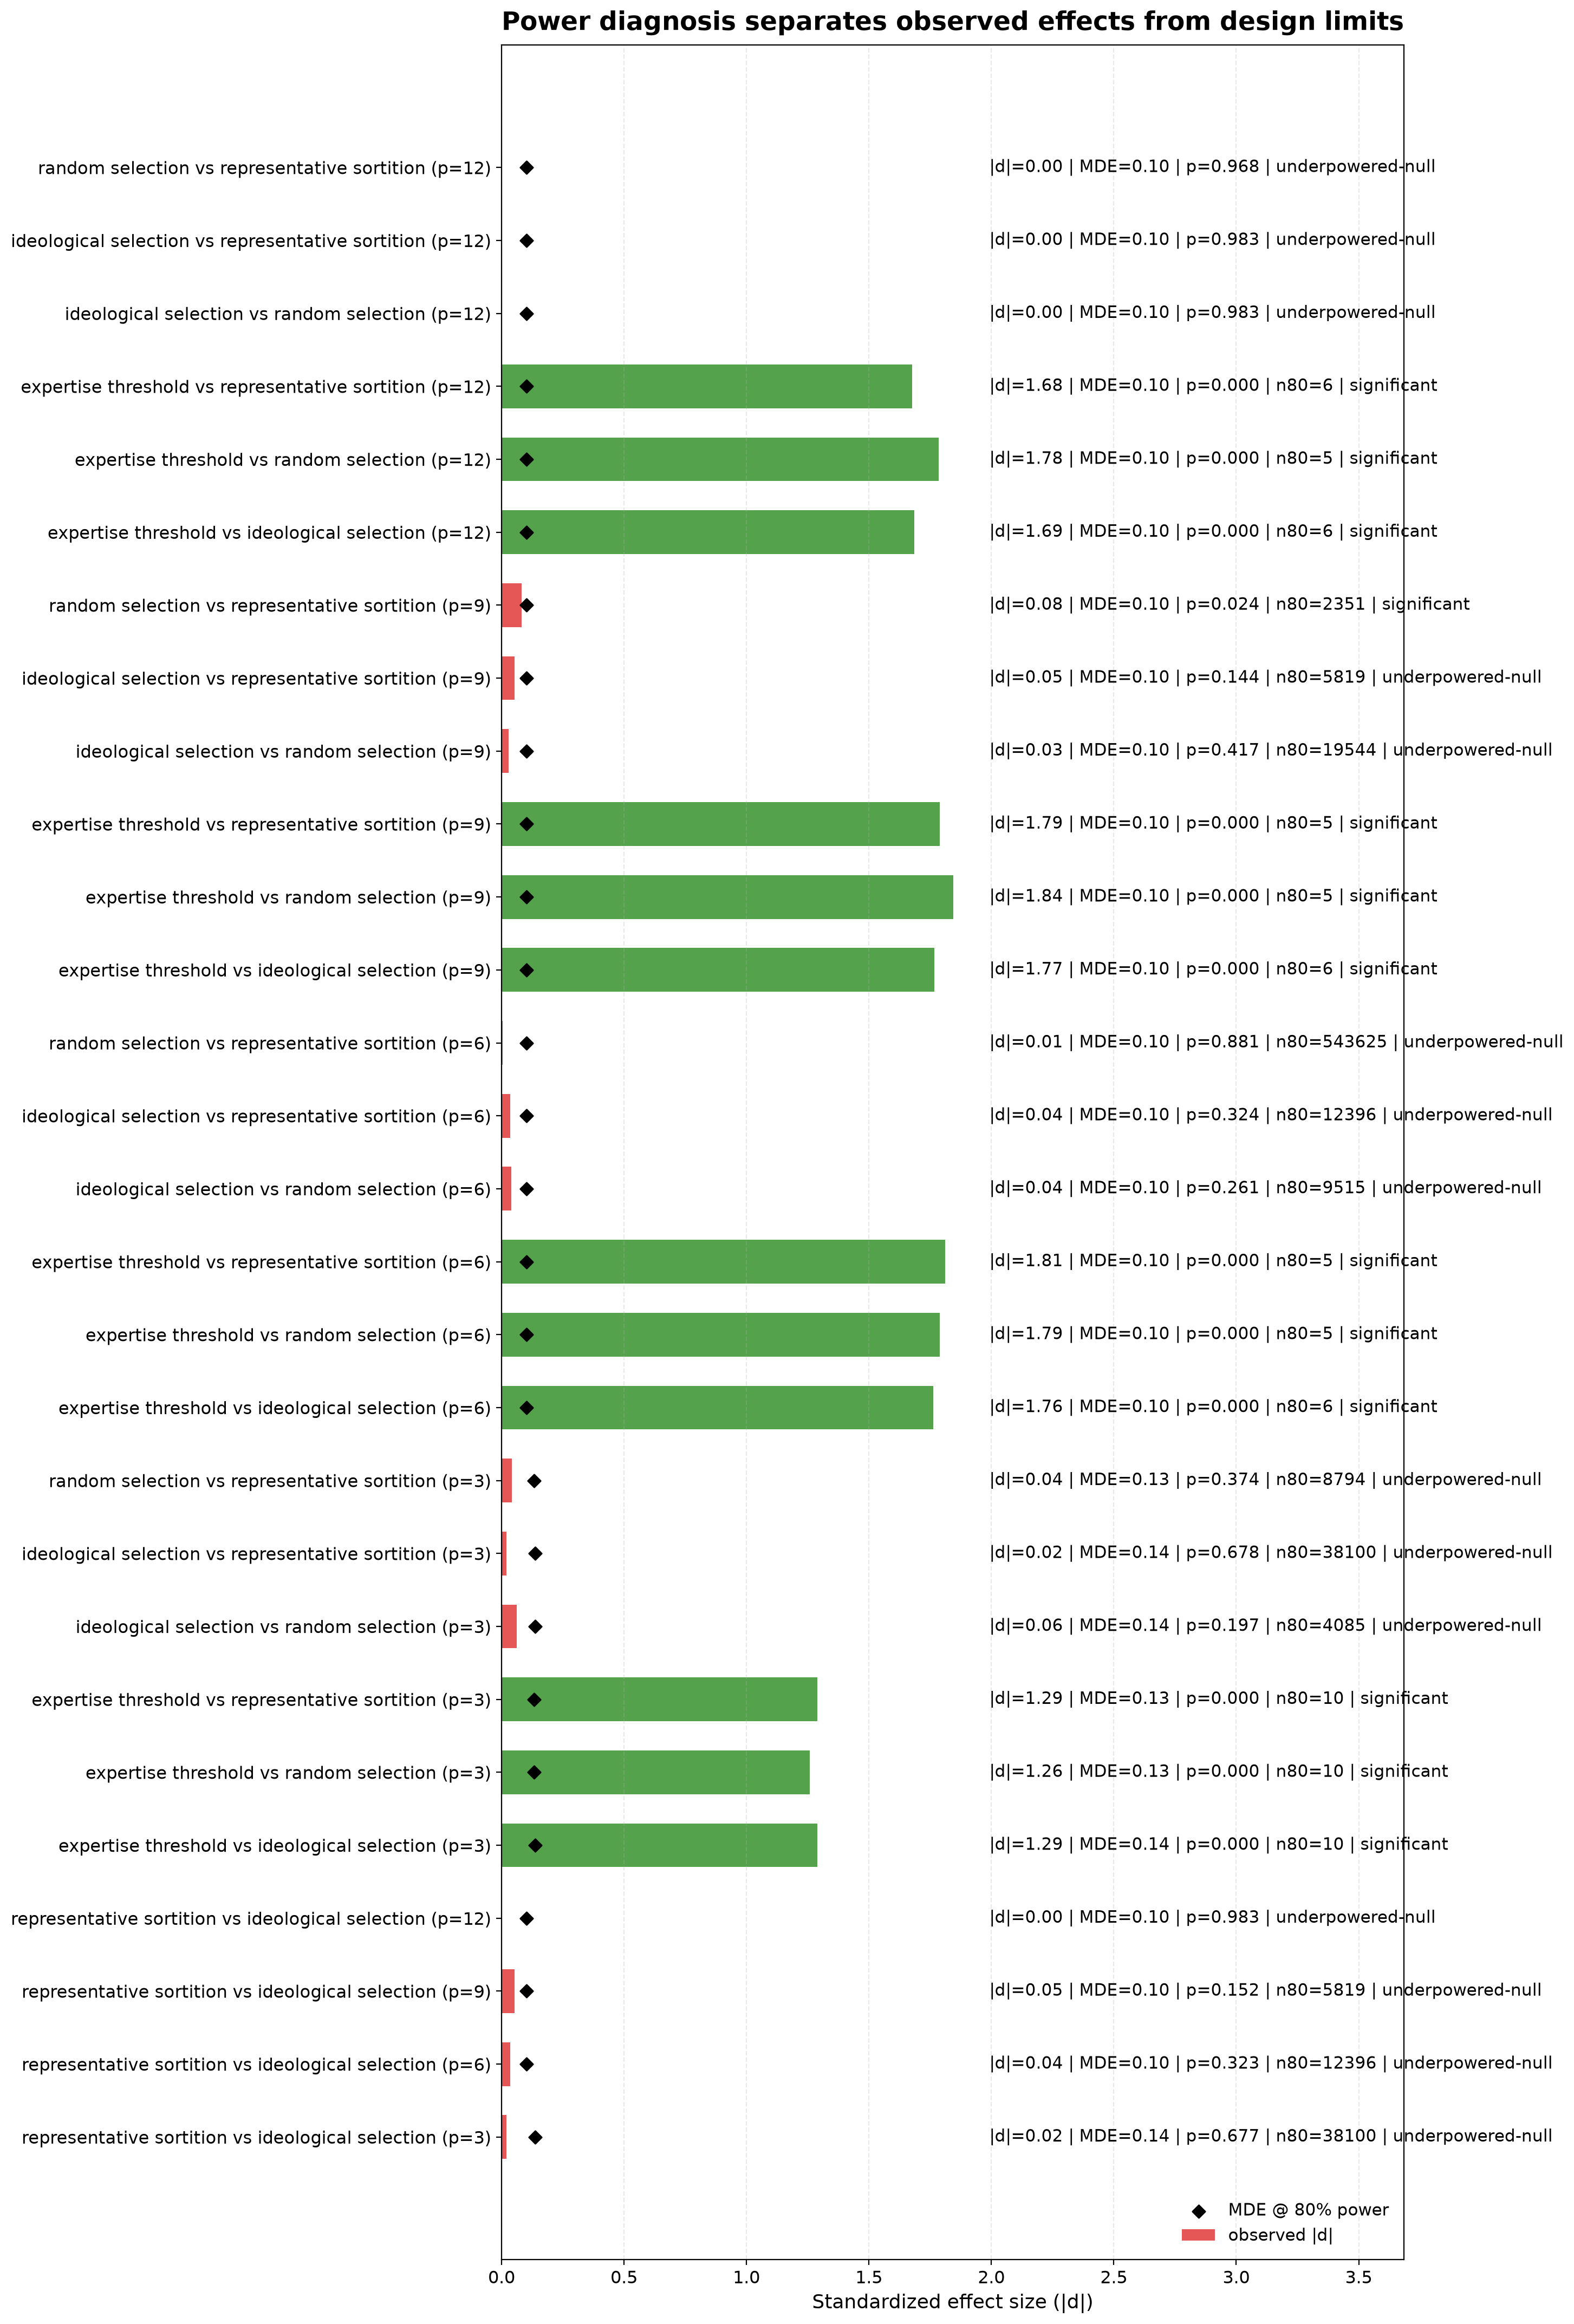
\includegraphics[width=0.8\linewidth,height=0.46\textheight,keepaspectratio,alt={Design-adequacy diagnosis for every pairwise strategy contrast, from source output/data/power\_analysis.csv: each row plots the observed standardized effect size (Cohen's d) against the minimum detectable effect (MDE) at 80\% power, annotated with the permutation p-value and the per-group observation budgets needed to resolve an effect of that size. A contrast whose observed \textbar d\textbar{} sits below its MDE marker is design-limited: the study could not have detected it even if it were real, so its non-significance is a statement about sample size, not about the absence of an effect. Claim: 16 of 28 contrasts are design-limited at the current observation count, which is why several neighboring-rank comparisons remain inconclusive; caveat: the budgets are keyed to the observed effect magnitudes and are prospective design targets, not retrospective observed power evidence.}]{../figures/power_design_diagnosis.png}
\caption{Design-adequacy diagnosis for every pairwise strategy contrast,
from source \protect\breaktt{output/data/power\_analysis.csv}: each row
plots the observed standardized effect size (Cohen's \(d\)) against the
minimum detectable effect (MDE) at 80\% power, annotated with the
permutation p-value and the per-group observation budgets needed to
resolve an effect of that size. A contrast whose observed \(|d|\) sits
below its MDE marker is design-limited: the study could not have
detected it even if it were real, so its non-significance is a statement
about sample size, not about the absence of an effect. Claim: 16 of 28
contrasts are design-limited at the current observation count, which is
why several neighboring-rank comparisons remain inconclusive; caveat:
the budgets are keyed to the observed effect magnitudes and are
prospective design targets, not retrospective observed power
evidence.}\label{fig:diagnosis}
\end{figure}

\begin{figure}
\centering
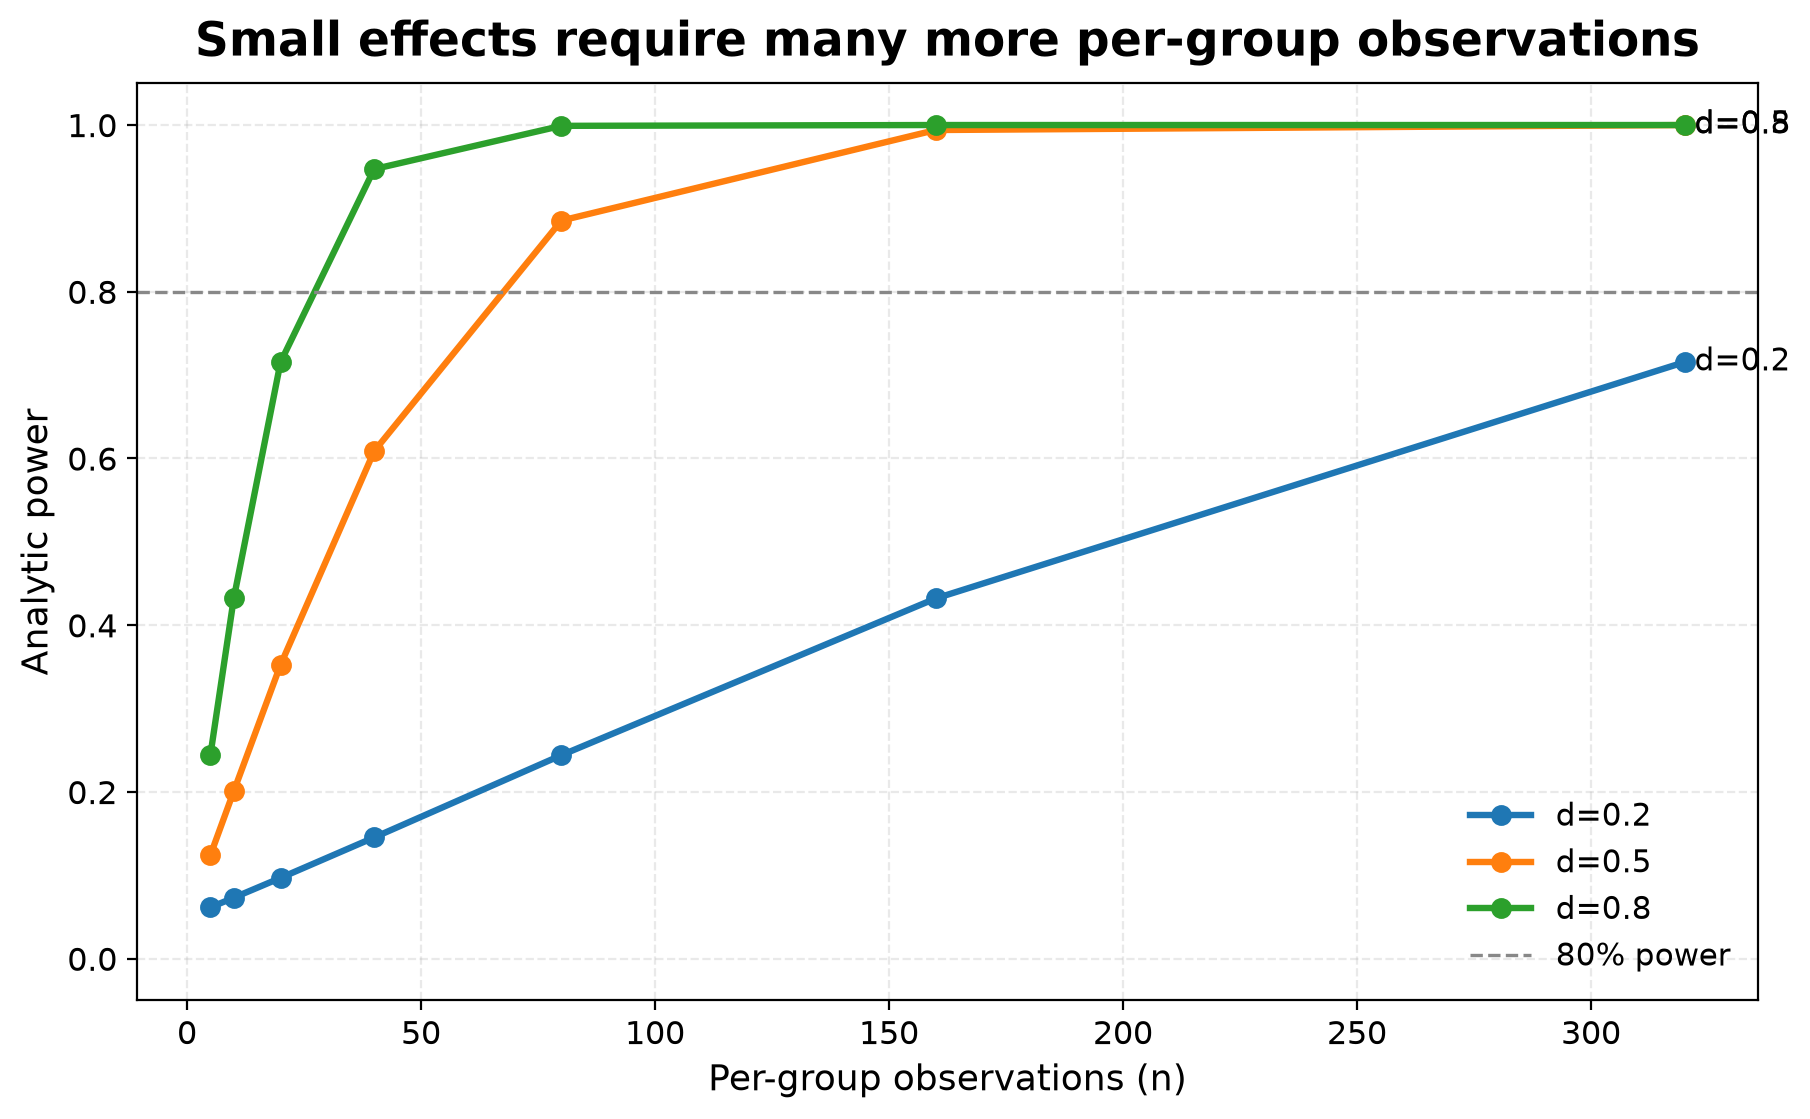
\includegraphics[width=0.72\linewidth,height=0.46\textheight,keepaspectratio,alt={Analytic two-sample power 1-\textbackslash beta (y-axis) versus samples-per-group n (x-axis, log scale), shown as a family of curves with one curve per representative Cohen's d value, computed from source output/data/power\_analysis.csv / src/ntqr\_allotment/power\_analysis.py; the horizontal dashed line marks the 80\% power target at the chosen \textbackslash alpha, and where each curve crosses it gives the n that effect size requires. Read it as a budgeting tool: the smaller the standardized effect, the further right its curve crosses the dashed line, i.e.~the more per-group observations are needed. Claim: small standardized effects require many more seeds per group than the current design provides, which is the mechanism behind the design-limited nulls; caveat: this is a prospective design-budget curve and an MDE visual, not retrospective observed power.}]{../figures/power_vs_n.png}
\caption{Analytic two-sample power \(1-\beta\) (y-axis) versus
samples-per-group \(n\) (x-axis, log scale), shown as a family of curves
with one curve per representative Cohen's \(d\) value, computed from
source \protect\breaktt{output/data/power\_analysis.csv} /
\protect\breaktt{src/ntqr\_allotment/power\_analysis.py}; the horizontal
dashed line marks the 80\% power target at the chosen \(\alpha\), and
where each curve crosses it gives the \(n\) that effect size requires.
Read it as a budgeting tool: the smaller the standardized effect, the
further right its curve crosses the dashed line, i.e.~the more per-group
observations are needed. Claim: small standardized effects require many
more seeds per group than the current design provides, which is the
mechanism behind the design-limited nulls; caveat: this is a prospective
design-budget curve and an MDE visual, not retrospective observed
power.}\label{fig:powervn}
\end{figure}

The remaining ``inconclusive'' verdicts are therefore statements about
\emph{design size}, made explicit through the minimum detectable effect
--- not evidence of no effect, and never reported as retrospective
observed power.
\end{block}

\begin{block}{Companion diagnostics bound cost, correlation, fairness,
and consistency}
\protect\phantomsection\label{companion-diagnostics-bound-cost-correlation-fairness-and-consistency}
The companion alarm's answer-key enumeration is roughly cubic in corpus
size (\breakseq{[@fig:alarm]}): about 0.7 s at \(Q=20\), 8.9 s at \(Q=50\), and
97.9 s at \(Q=100\) (measured by \breaktt{scripts/bench\_alarm.py},
written to \breaktt{output/data/alarm\_timings.csv}). This is a real
ceiling on the alarm track, so it is opt-in and capped at \(Q\leq30\).
We report it as a finding: the alarm is usable as a small-corpus
consistency check, not as a sweep-scale primitive.

\begin{figure}
\centering
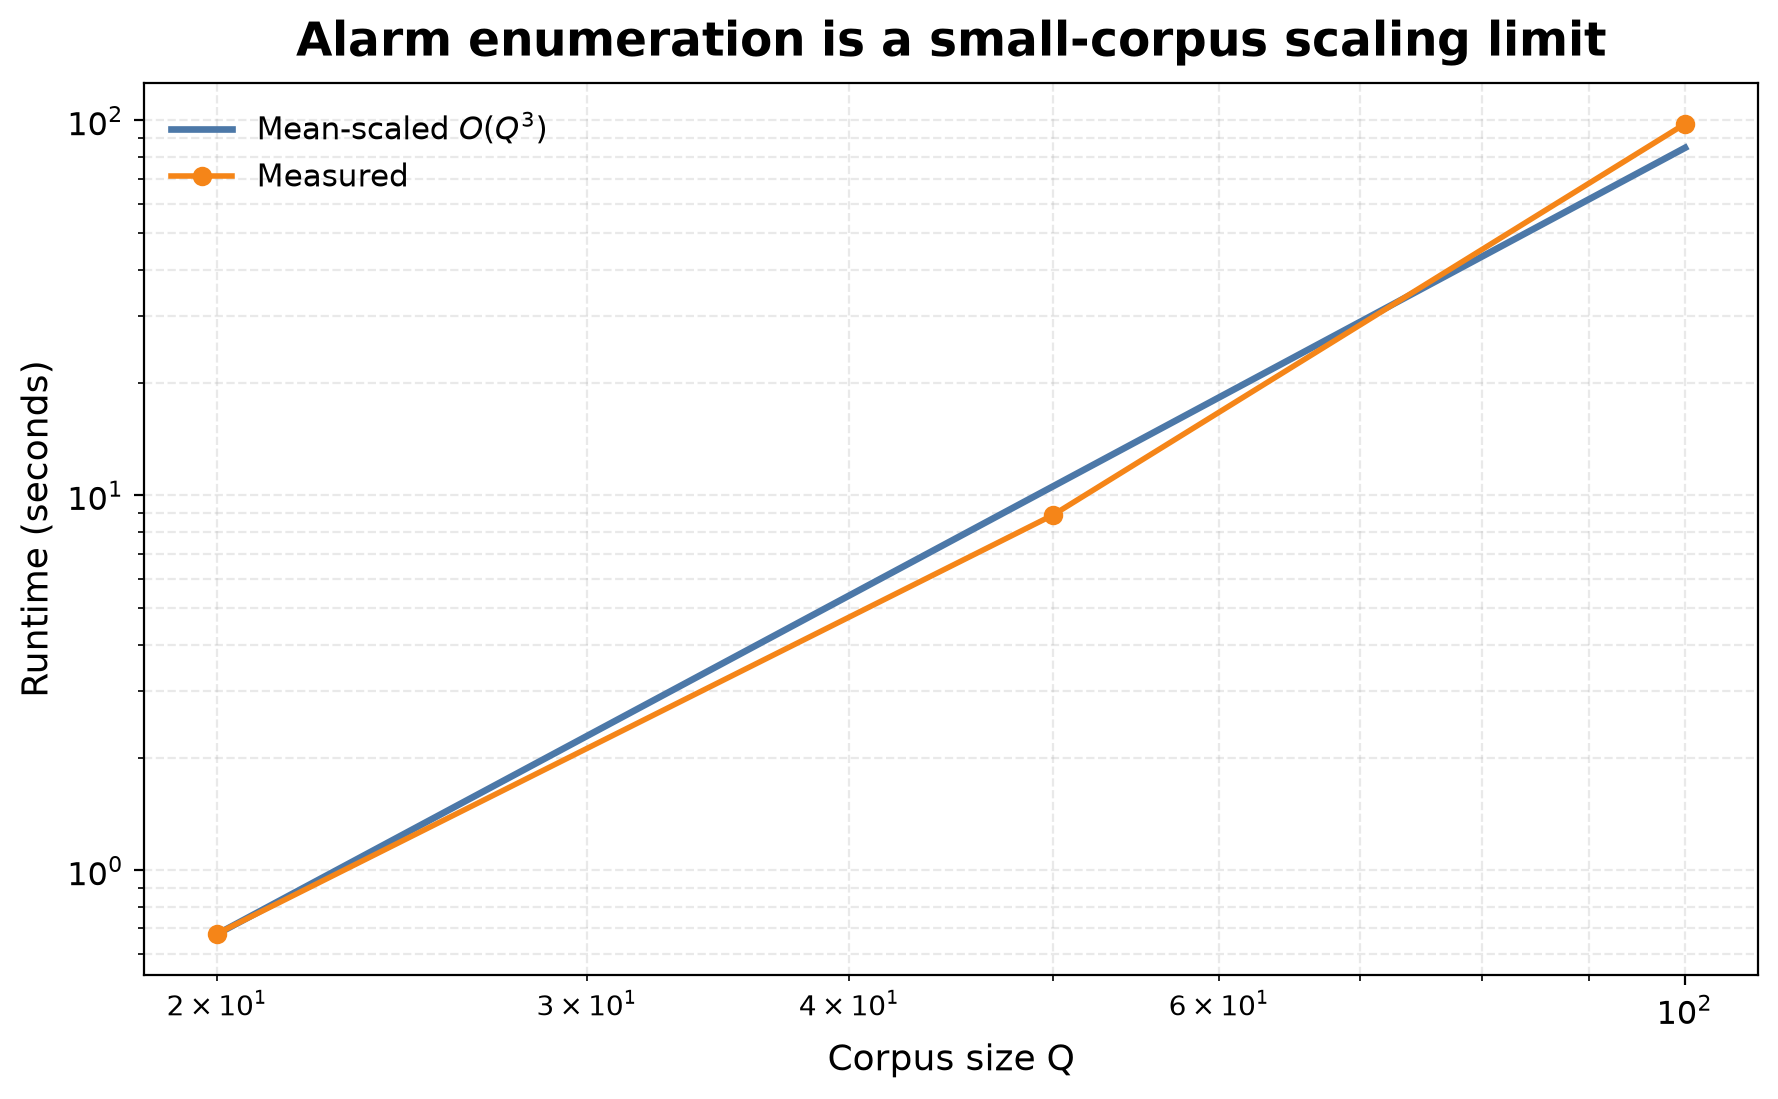
\includegraphics[width=0.7\linewidth,height=0.46\textheight,keepaspectratio,alt={Measured alarm wall-clock time (seconds) versus corpus size Q on log-log axes, from source output/data/alarm\_timings.csv, with a cubic O(Q\^{}3) reference line overlaid. On log-log axes a power law is a straight line whose slope is its exponent, so the measured points tracking the reference slope is the visual evidence that the answer-key-enumeration alarm scales cubically in Q. The practical consequence is a hard ceiling: the wall-clock cost rises steeply enough that the alarm is usable only as a small-corpus consistency check. Claim: at the current implementation the alarm is small-corpus only and is therefore opt-in and capped; caveat: the absolute wall-clock constants are machine-local and load-dependent, so it is the cubic scaling, not the individual timings, that is the robust finding.}]{../figures/alarm_cost_curve.png}
\caption{Measured alarm wall-clock time (seconds) versus corpus size
\(Q\) on log-log axes, from source
\protect\breaktt{output/data/alarm\_timings.csv}, with a cubic \(O(Q^3)\)
reference line overlaid. On log-log axes a power law is a straight line
whose slope is its exponent, so the measured points tracking the
reference slope is the visual evidence that the answer-key-enumeration
alarm scales cubically in \(Q\). The practical consequence is a hard
ceiling: the wall-clock cost rises steeply enough that the alarm is
usable only as a small-corpus consistency check. Claim: at the current
implementation the alarm is small-corpus only and is therefore opt-in
and capped; caveat: the absolute wall-clock constants are machine-local
and load-dependent, so it is the cubic scaling, not the individual
timings, that is the robust finding.}\label{fig:alarm}
\end{figure}

Three further companion tracks measure structural properties of the
pipeline rather than recovery error, and we report them as diagnostics.
The error-correlation track records the mean realized correlation each
formation strategy induces (\breakseq{[@fig:strategycorr]}): single-bloc
selection sits highest, consistent with its status as the deliberately
correlated comparator. The maximin fairness track characterizes the
representative lottery's selection-probability distribution over the
population (\breakseq{[@fig:fairness]}) --- the maximin objective is the floor
on who can be seated, independent of any downstream recovery number. The
N-judge alarm-power track records a saturated small-\(Q\) alarm-firing
rate across the plotted panel sizes (\breakseq{[@fig:alarmpower]}). The ternary
(\(R=3\)) track is consistency/feasibility only --- it confirms
three-way vote profiles satisfy the NTQR axioms and is never an \(R=3\)
recovery claim (out of scope) --- so it yields a pass/fail check rather
than a plotted number.

\begin{figure}
\centering
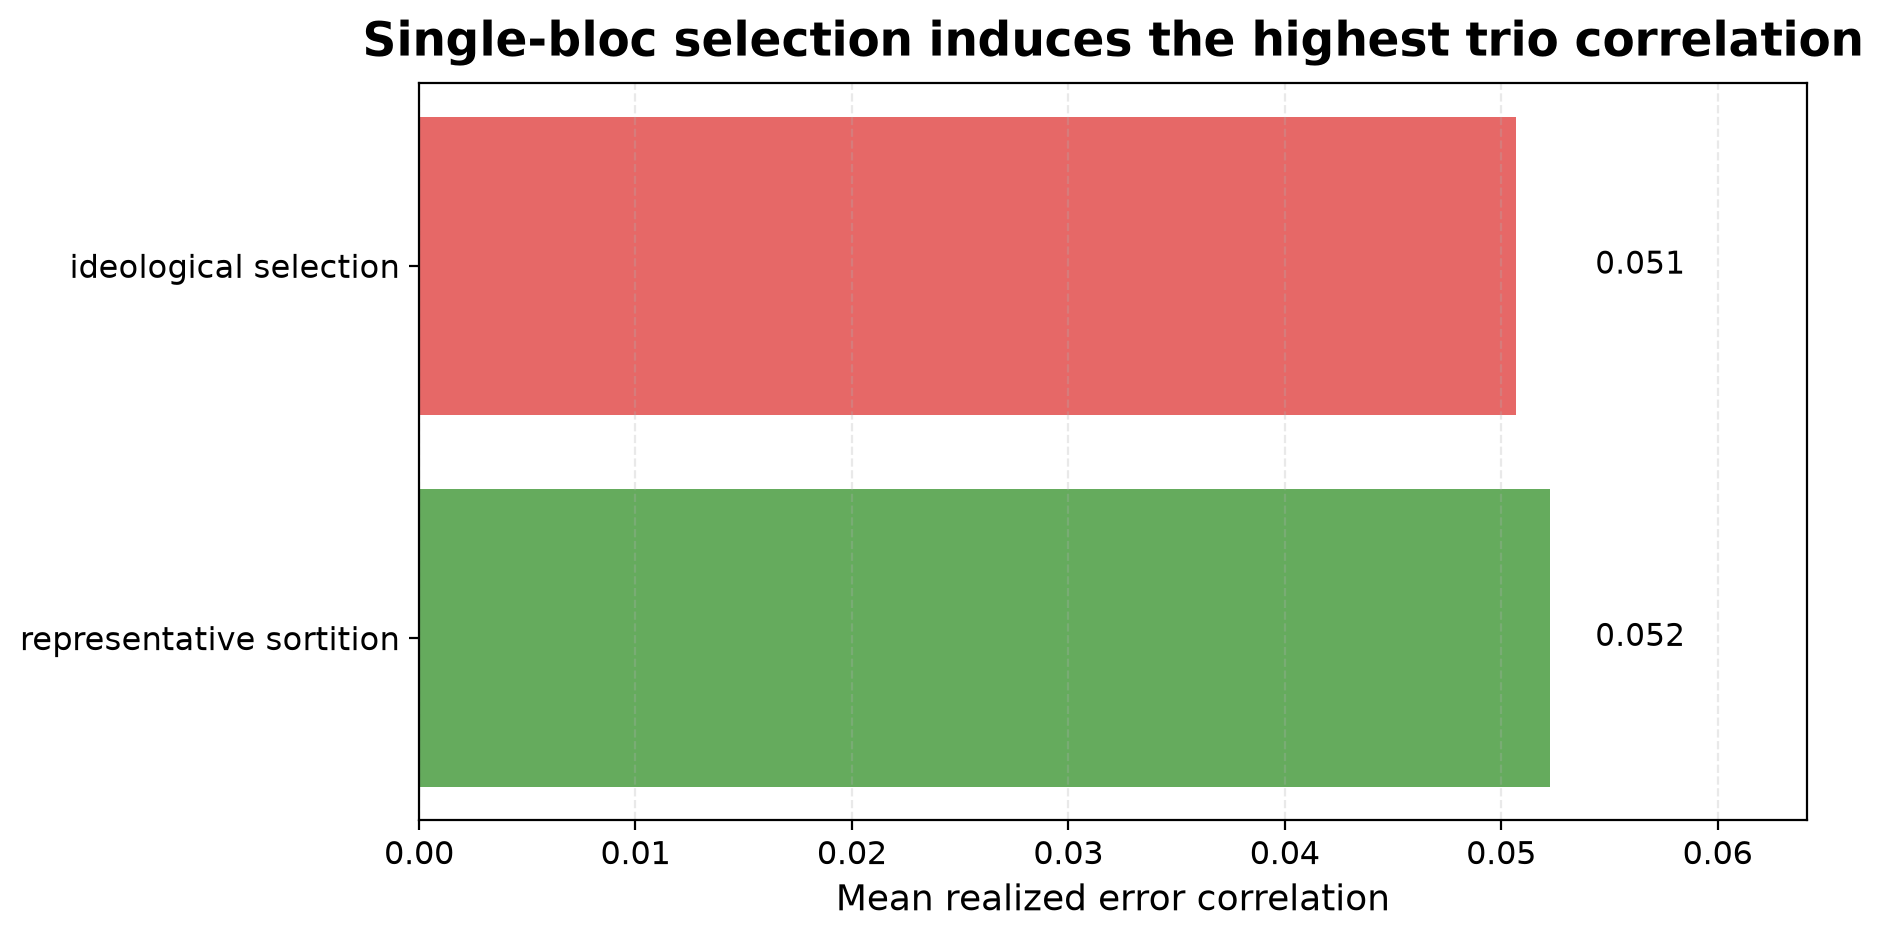
\includegraphics[width=0.7\linewidth,height=0.46\textheight,keepaspectratio,alt={Bar chart of the mean realized pairwise error correlation that each panel-formation strategy induces among its judges, measured by NTQR's own supervised estimator over the tolerance sweep, from source output/data/independence\_sweep.csv. Higher bars mean the strategy seats judges whose mistakes are more correlated, which is precisely the error-independence assumption the exact trio solver leans on. Single-bloc selection is the tallest bar, consistent with its design as the deliberately correlated comparator, while representative and random draws sit lower. Read this as a structural property of the draw itself, upstream of any recovery number. Caveat: this is a structural diagnostic of the formed panel, not a recovery-effect claim about downstream EIE error.}]{../figures/strategy_correlation.png}
\caption{Bar chart of the mean realized pairwise error correlation that
each panel-formation strategy induces among its judges, measured by
NTQR's own supervised estimator over the tolerance sweep, from source
\protect\breaktt{output/data/independence\_sweep.csv}. Higher bars mean
the strategy seats judges whose mistakes are more correlated, which is
precisely the error-independence assumption the exact trio solver leans
on. Single-bloc selection is the tallest bar, consistent with its design
as the deliberately correlated comparator, while representative and
random draws sit lower. Read this as a structural property of the draw
itself, upstream of any recovery number. Caveat: this is a structural
diagnostic of the formed panel, not a recovery-effect claim about
downstream EIE error.}\label{fig:strategycorr}
\end{figure}

\begin{figure}
\centering
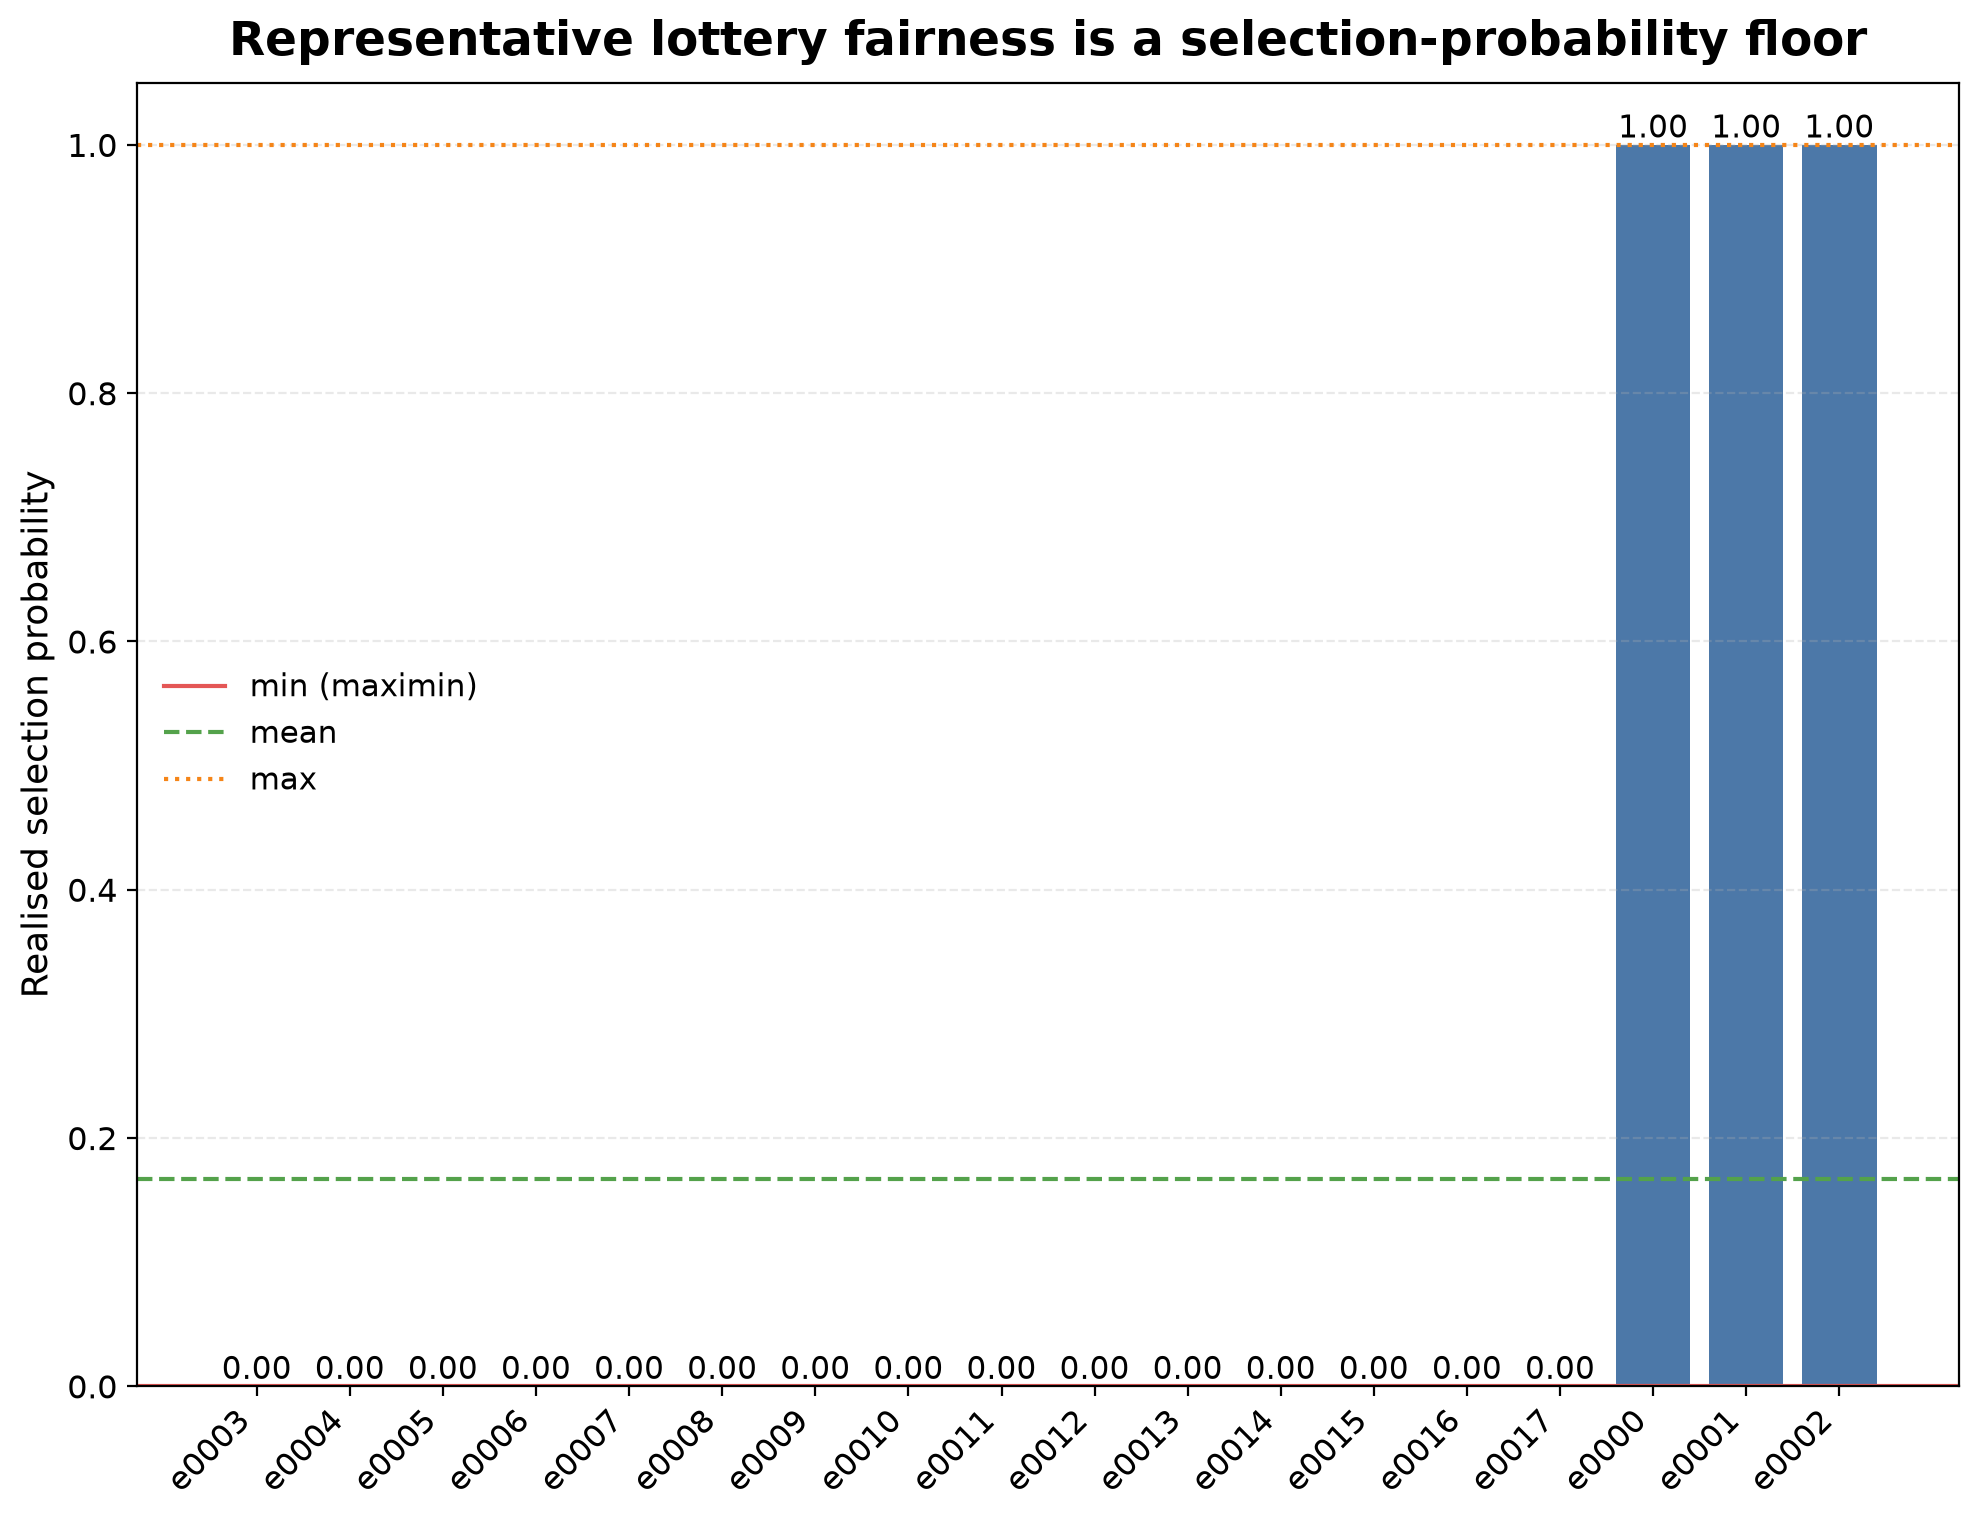
\includegraphics[width=0.7\linewidth,height=0.46\textheight,keepaspectratio,alt={Per-candidate selection probabilities under the representative maximin sortition lottery, computed from src/ntqr\_allotment/fairness.py over the feasible panel draws. Each bar is one expert's probability of being seated across the lottery; the maximin objective explicitly maximises the smallest of these probabilities, so the figure should be read by its floor (the shortest bar) rather than its average --- a fairer lottery lifts the worst-off candidate's chance of selection. This characterises the representation properties of the draw and is fully independent of any downstream evaluation number. Caveat: this describes panel-formation fairness only, not NTQR recovery error.}]{../figures/fairness_maximin.png}
\caption{Per-candidate selection probabilities under the representative
maximin sortition lottery, computed from
\protect\breaktt{src/ntqr\_allotment/fairness.py} over the feasible panel
draws. Each bar is one expert's probability of being seated across the
lottery; the maximin objective explicitly maximises the smallest of
these probabilities, so the figure should be read by its floor (the
shortest bar) rather than its average --- a fairer lottery lifts the
worst-off candidate's chance of selection. This characterises the
representation properties of the draw and is fully independent of any
downstream evaluation number. Caveat: this describes panel-formation
fairness only, not NTQR recovery error.}\label{fig:fairness}
\end{figure}

\begin{figure}
\centering
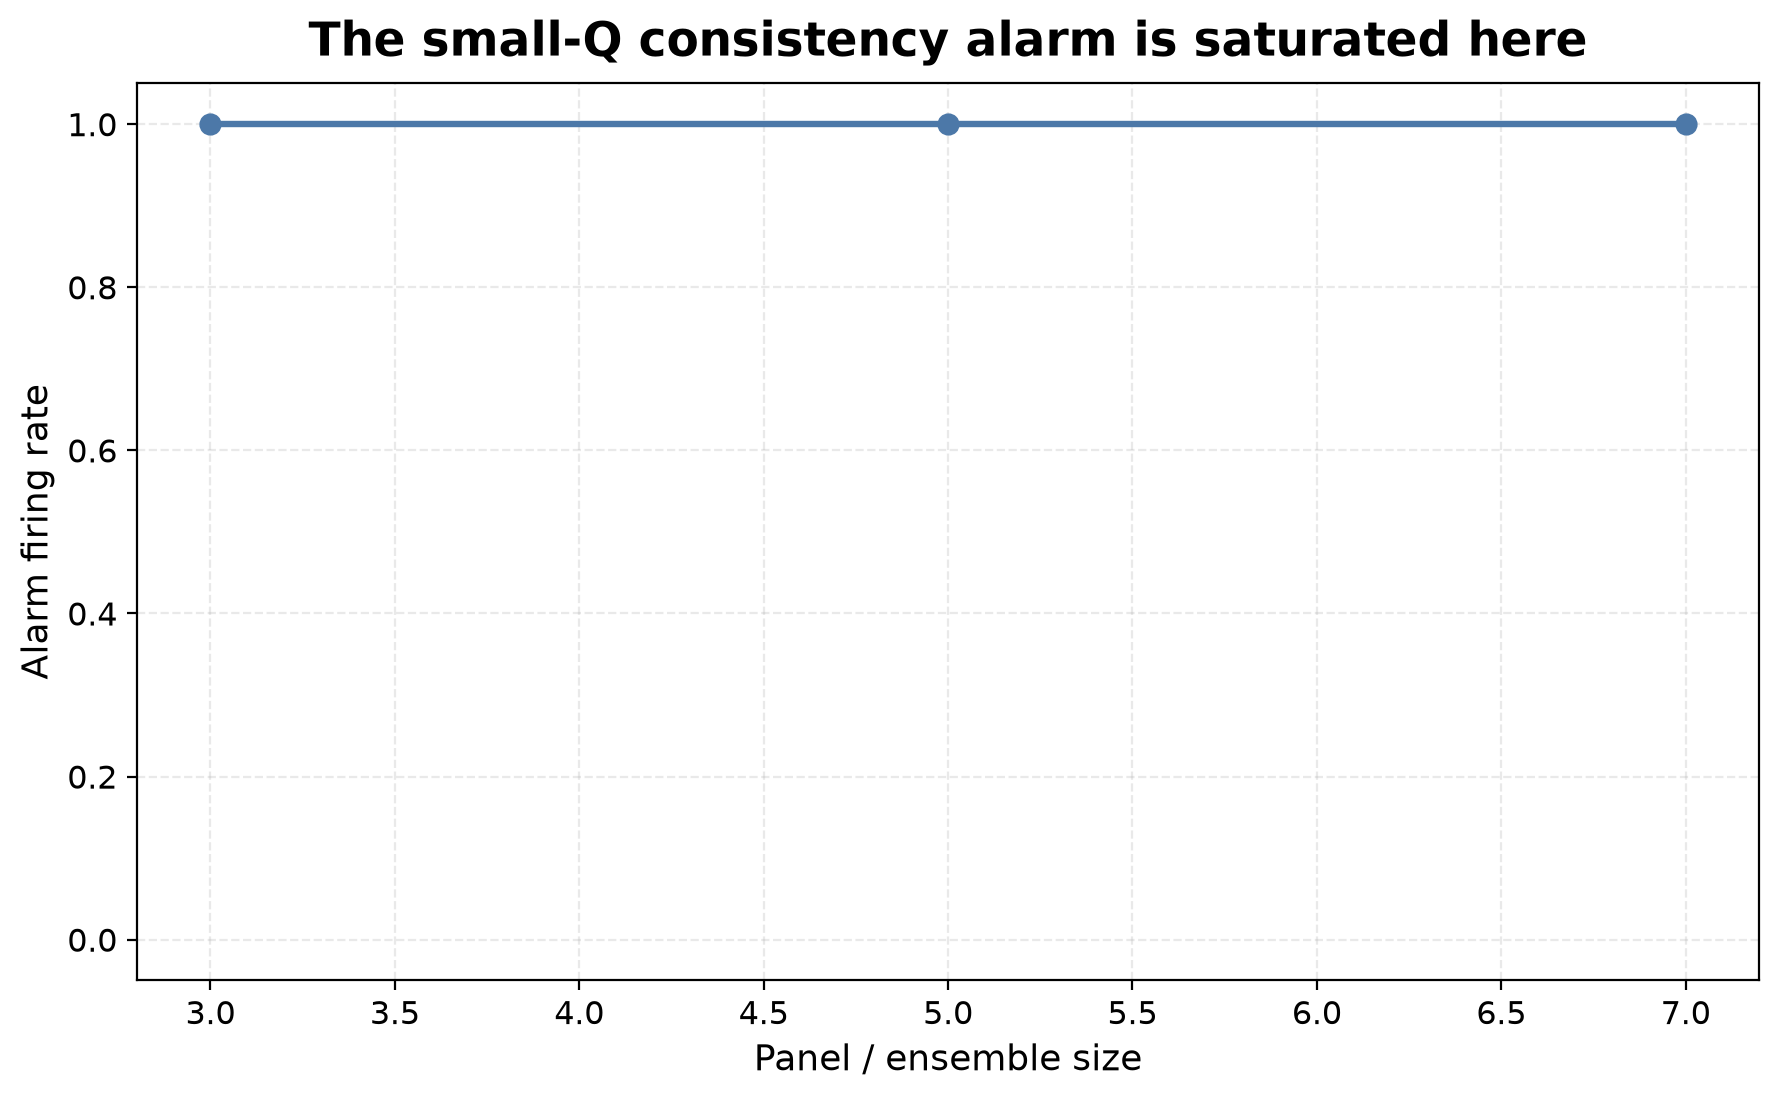
\includegraphics[width=0.7\linewidth,height=0.46\textheight,keepaspectratio,alt={N-judge alarm firing rate as a function of panel size at small corpus size Q, computed live from src/ntqr\_allotment/ensemble.py. The alarm fires when no single answer key can make all seated judges simultaneously axiom-consistent at the stated safety specification; the curve shows how often that happens as the panel grows. At the tight safety setting plotted here the rate is already saturated across the panel sizes shown, so the figure demonstrates that the N-judge alarm is executable and panel-size-indexed rather than establishing a monotone growth law (a looser setting would be needed to see a rising curve). Caveat: the alarm track is a consistency signal only, never a recovery method, and is bounded by the same O(Q\^{}3) answer-key enumeration, which confines it to small Q.}]{../figures/alarm_power.png}
\caption{N-judge alarm firing rate as a function of panel size at small
corpus size \(Q\), computed live from
\protect\breaktt{src/ntqr\_allotment/ensemble.py}. The alarm fires when
no single answer key can make all seated judges simultaneously
axiom-consistent at the stated safety specification; the curve shows how
often that happens as the panel grows. At the tight safety setting
plotted here the rate is already saturated across the panel sizes shown,
so the figure demonstrates that the N-judge alarm is executable and
panel-size-indexed rather than establishing a monotone growth law (a
looser setting would be needed to see a rising curve). Caveat: the alarm
track is a consistency signal only, never a recovery method, and is
bounded by the same \(O(Q^3)\) answer-key enumeration, which confines it
to small \(Q\).}\label{fig:alarmpower}
\end{figure}

\clearpage
\end{block}
\end{frame}

\begin{frame}[fragile,allowframebreaks]{Real-Ollama postdoctoral panel
results: live H5 companion}
\protect\phantomsection\label{real-ollama-postdoctoral-panel-results-live-h5-companion}
The live-Ollama results are separate empirical companion artifacts. They
use one local \texttt{gemma3:4b} model prompted as synthetic
postdoctoral reviewers over fictitious applications with synthetic age
metadata. The result is not a model-family comparison, not a
human-review validation, and not evidence that age belongs in real
admissions or hiring review.

\begin{block}{Gemma ranking asks the same sampling question under prompt
labels}
\protect\phantomsection\label{gemma-ranking-asks-the-same-sampling-question-under-prompt-labels}
The live artifact uses 12 seeds, 48 reviewers, 72 applications per seed,
panel sizes 3, 6, and live Ollama provenance (\texttt{gemma3:4b} digest
a2af6cc3eb7f, config hash 5161ffe474b3, vote-cache entries 23688). The
best live postdoc EIE point estimate is same-bias selection at 0.216;
the worst is expertise threshold at 0.347. For the three-seat panels,
representative sortition has EIE 0.225, same-bias selection has 0.228,
expertise-threshold selection has 0.347, and random selection has 0.262.

\begin{figure}
\centering
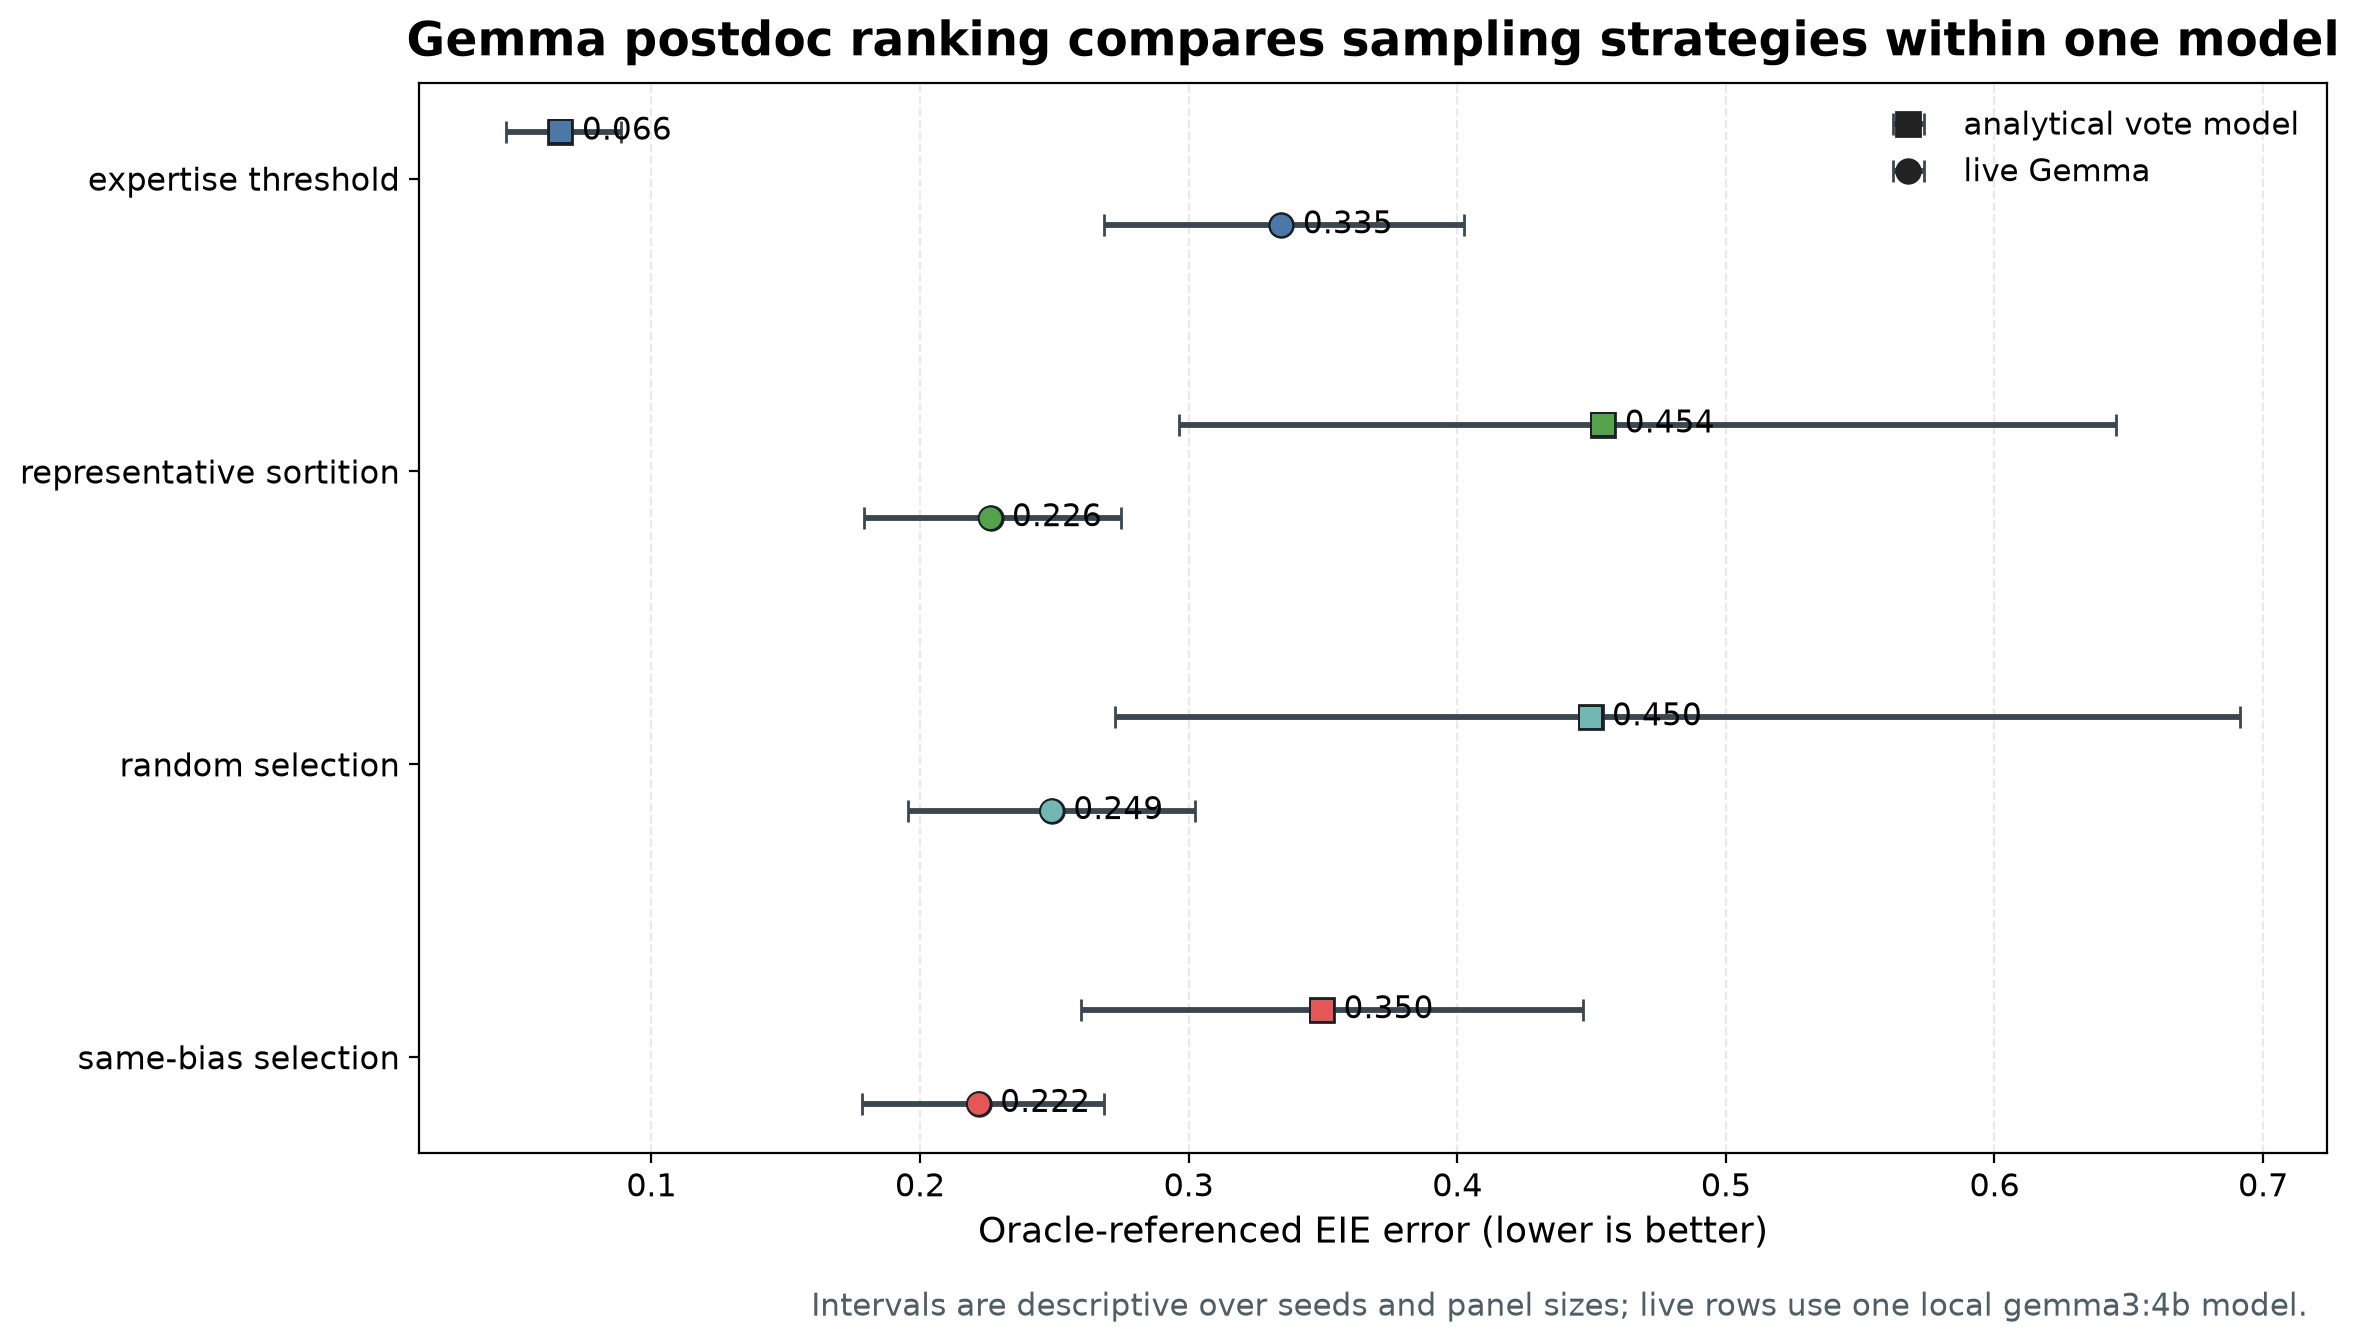
\includegraphics[width=0.8\linewidth,height=0.46\textheight,keepaspectratio,alt={Side-by-side strategy ranking for the analytical vote model (square markers) and the live Gemma reviewer panel (circle markers), one row per sampling strategy, from source output/data/postdoc\_panel\_results.json. Metric: oracle-referenced EIE error (lower is better), aggregated by track, sampling strategy, and panel size, with descriptive intervals over 12 seeds. The two marker shapes are juxtaposed, never pooled, so the reader can see where the live model echoes the analytical ordering and where it departs; the horizontal gap between a strategy's square and circle is exactly that analytical-vs-live divergence. Claim: the live single-model panel is analysed as a within-model sampling-strategy stress test, not as an LLM-family comparison; caveat: it uses synthetic applications and age metadata only, one local Gemma model, and carries no human-review validation.}]{../figures/postdoc_strategy_ranking.png}
\caption{Side-by-side strategy ranking for the analytical vote model
(square markers) and the live Gemma reviewer panel (circle markers), one
row per sampling strategy, from source
\protect\breaktt{output/data/postdoc\_panel\_results.json}. Metric:
oracle-referenced EIE error (lower is better), aggregated by track,
sampling strategy, and panel size, with descriptive intervals over 12
seeds. The two marker shapes are juxtaposed, never pooled, so the reader
can see where the live model echoes the analytical ordering and where it
departs; the horizontal gap between a strategy's square and circle is
exactly that analytical-vs-live divergence. Claim: the live single-model
panel is analysed as a within-model sampling-strategy stress test, not
as an LLM-family comparison; caveat: it uses synthetic applications and
age metadata only, one local Gemma model, and carries no human-review
validation.}\label{fig:postdocrank}
\end{figure}
\end{block}

\begin{block}{Same-bias panels expose age-conditioned recommendations}
\protect\phantomsection\label{same-bias-panels-expose-age-conditioned-recommendations}
The age-bias outcome is older-minus-younger recommendation rate.
Positive values mean older synthetic applicants are recommended more
often; negative values mean younger synthetic applicants are recommended
more often. At the three-seat panel grain, representative sortition's
live disparity is -0.190, while same-bias selection's live disparity is
-0.214. Age bias here \emph{is} simply illegitimate: because true
quality is generated independently of age, any age-conditioned shift is
a reviewer acting on an irrelevant attribute. That is exactly why age is
a useful \emph{probe} --- it gives a clean, known-illegitimate signal
whose magnitude we can read directly --- so the question is not whether
age bias is acceptable (it is not) but whether the upstream sampling
rule \textbf{amplifies or contains} an illegitimate bias the reviewers
already carry. The disparities here are negative across the board,
meaning this model favors younger synthetic applicants; the experiment
measures that illegitimate behavior to compare bias containment across
sampling rules (age is a probe; see Ethics).

\begin{figure}
\centering
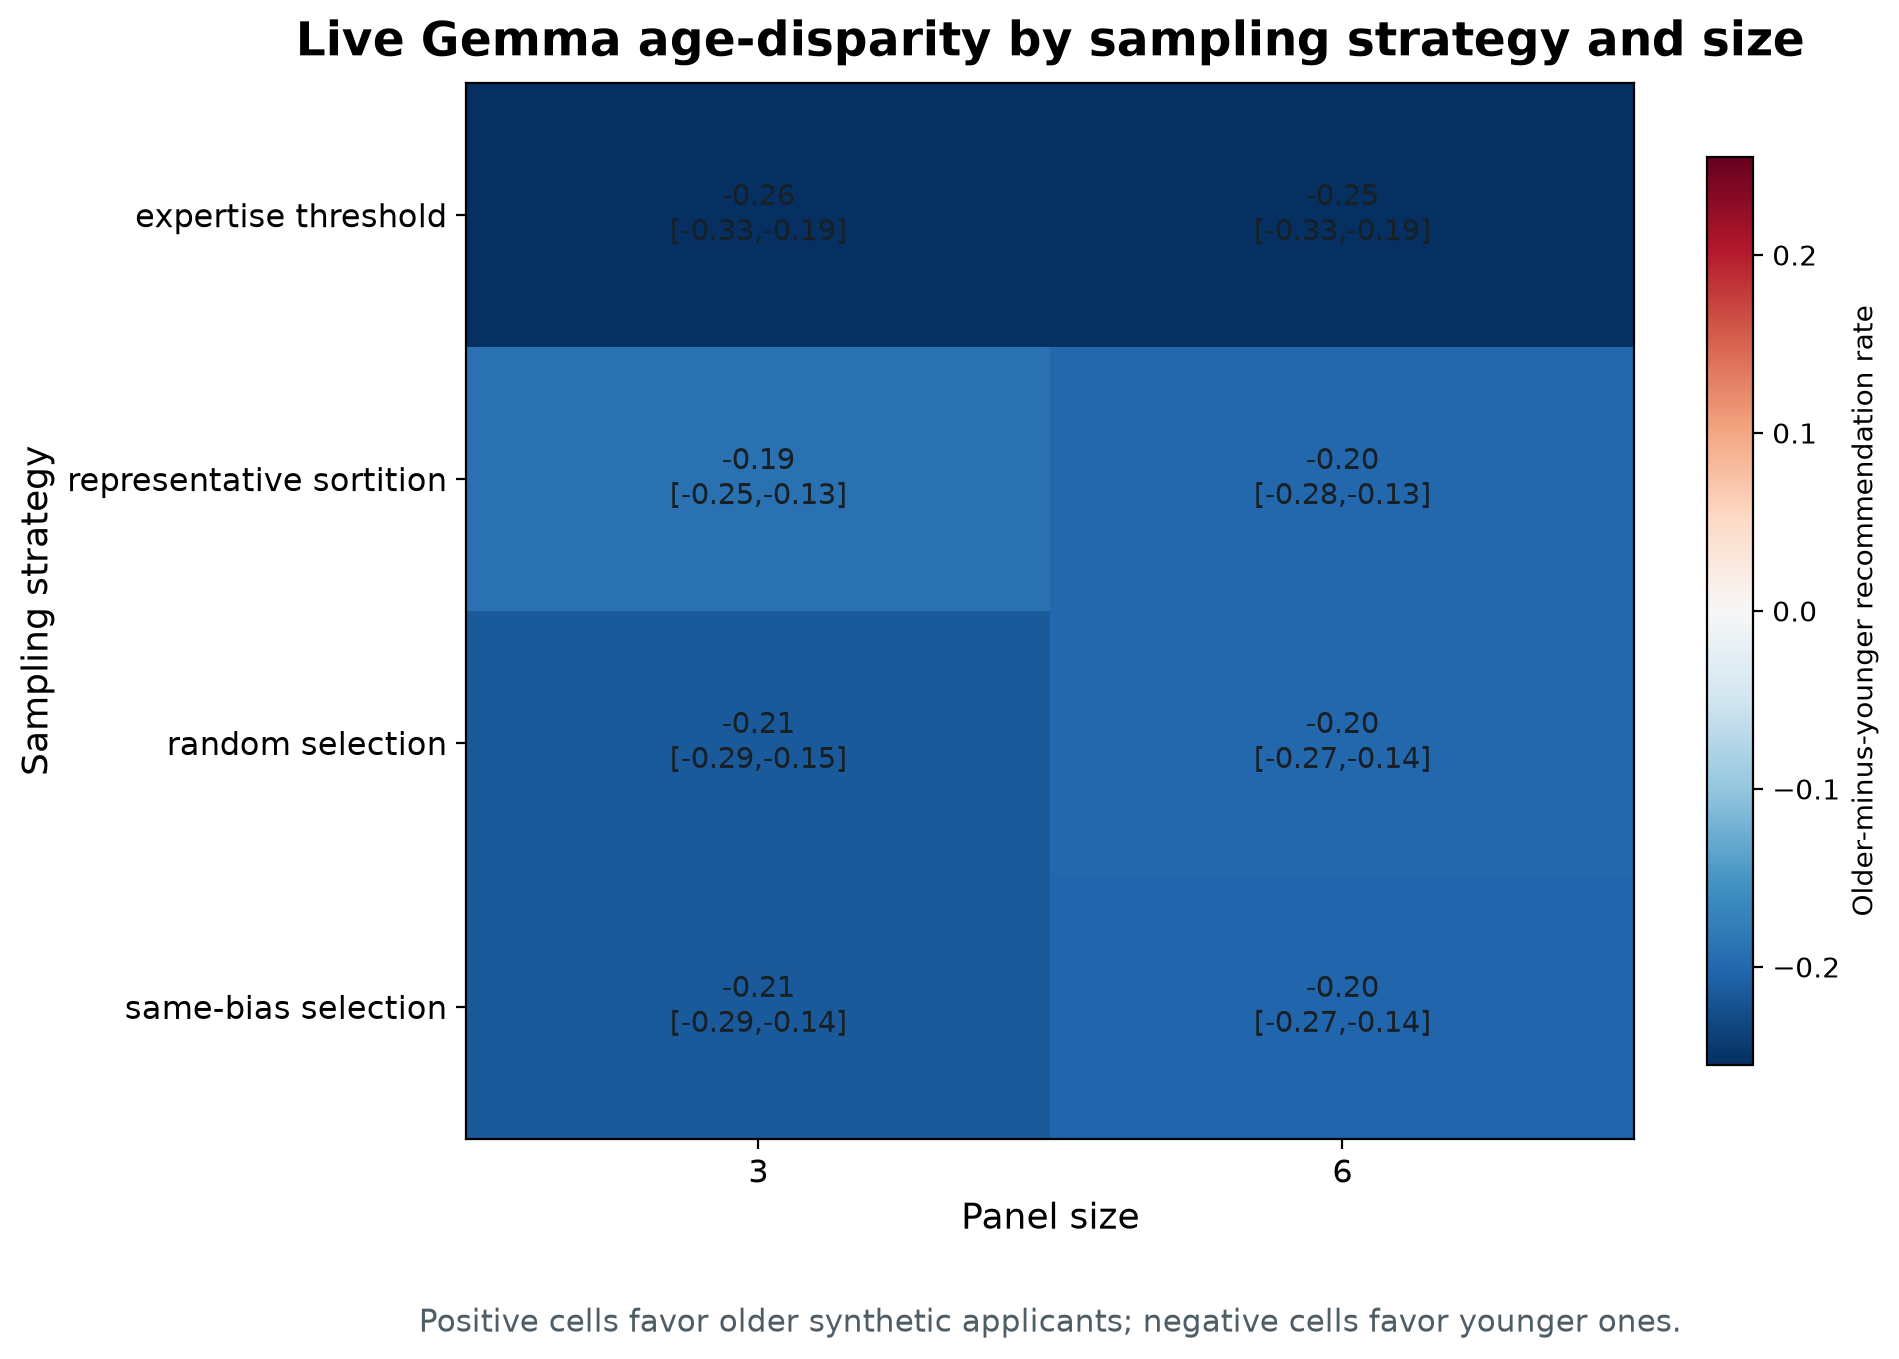
\includegraphics[width=0.72\linewidth,height=0.46\textheight,keepaspectratio,alt={Heatmap of the older-minus-younger recommendation-rate disparity expressed by the live Gemma reviewer panel, by sampling strategy (rows) and panel size (columns), from source output/data/postdoc\_panel\_results.json. Because true latent quality is generated independently of age, any non-zero cell is reviewer age-bias expression rather than signal: positive values mean older synthetic applicants are recommended more often, negative values mean younger applicants are. Metric: age-conditioned recommendation-rate difference, aggregated over 12 seeds; read down a column to compare how each sampling rule amplifies or dampens the irrelevant age signal. Claim: same-bias (single-bloc) sampling is the explicit bias-amplification stress test among the strategies; caveat: all applicants and ages are synthetic, and this figure does not validate Gemma or endorse age-aware real review.}]{../figures/postdoc_age_bias_heatmap.png}
\caption{Heatmap of the older-minus-younger recommendation-rate
disparity expressed by the live Gemma reviewer panel, by sampling
strategy (rows) and panel size (columns), from source
\protect\breaktt{output/data/postdoc\_panel\_results.json}. Because true
latent quality is generated independently of age, any non-zero cell is
reviewer age-bias expression rather than signal: positive values mean
older synthetic applicants are recommended more often, negative values
mean younger applicants are. Metric: age-conditioned recommendation-rate
difference, aggregated over 12 seeds; read down a column to compare how
each sampling rule amplifies or dampens the irrelevant age signal.
Claim: same-bias (single-bloc) sampling is the explicit
bias-amplification stress test among the strategies; caveat: all
applicants and ages are synthetic, and this figure does not validate
Gemma or endorse age-aware real review.}\label{fig:postdocbias}
\end{figure}
\end{block}

\begin{block}{Analytical and Gemma cells stay juxtaposed, not pooled}
\protect\phantomsection\label{analytical-and-gemma-cells-stay-juxtaposed-not-pooled}
The alignment artifact compares analytical prediction signs with live
Gemma observations by strategy and panel size. 8 of 8 cells are resolved
after zero-sign cells are marked unresolved; the resolved-cell
sign-agreement rate is 0.500. This agreement is a \textbf{weak
directional check, not an independent match}: every live Gemma
age-disparity sign in this run is negative (the model uniformly favors
younger synthetic applicants), so the rate mostly measures how often the
analytical sign is also negative rather than a cell-by-cell coincidence
of two freely varying signals. This is the intended bridge between the
synthetic and live tracks: same causal question, shared sampling
vocabulary, separate evidence levels.

\begin{figure}
\centering
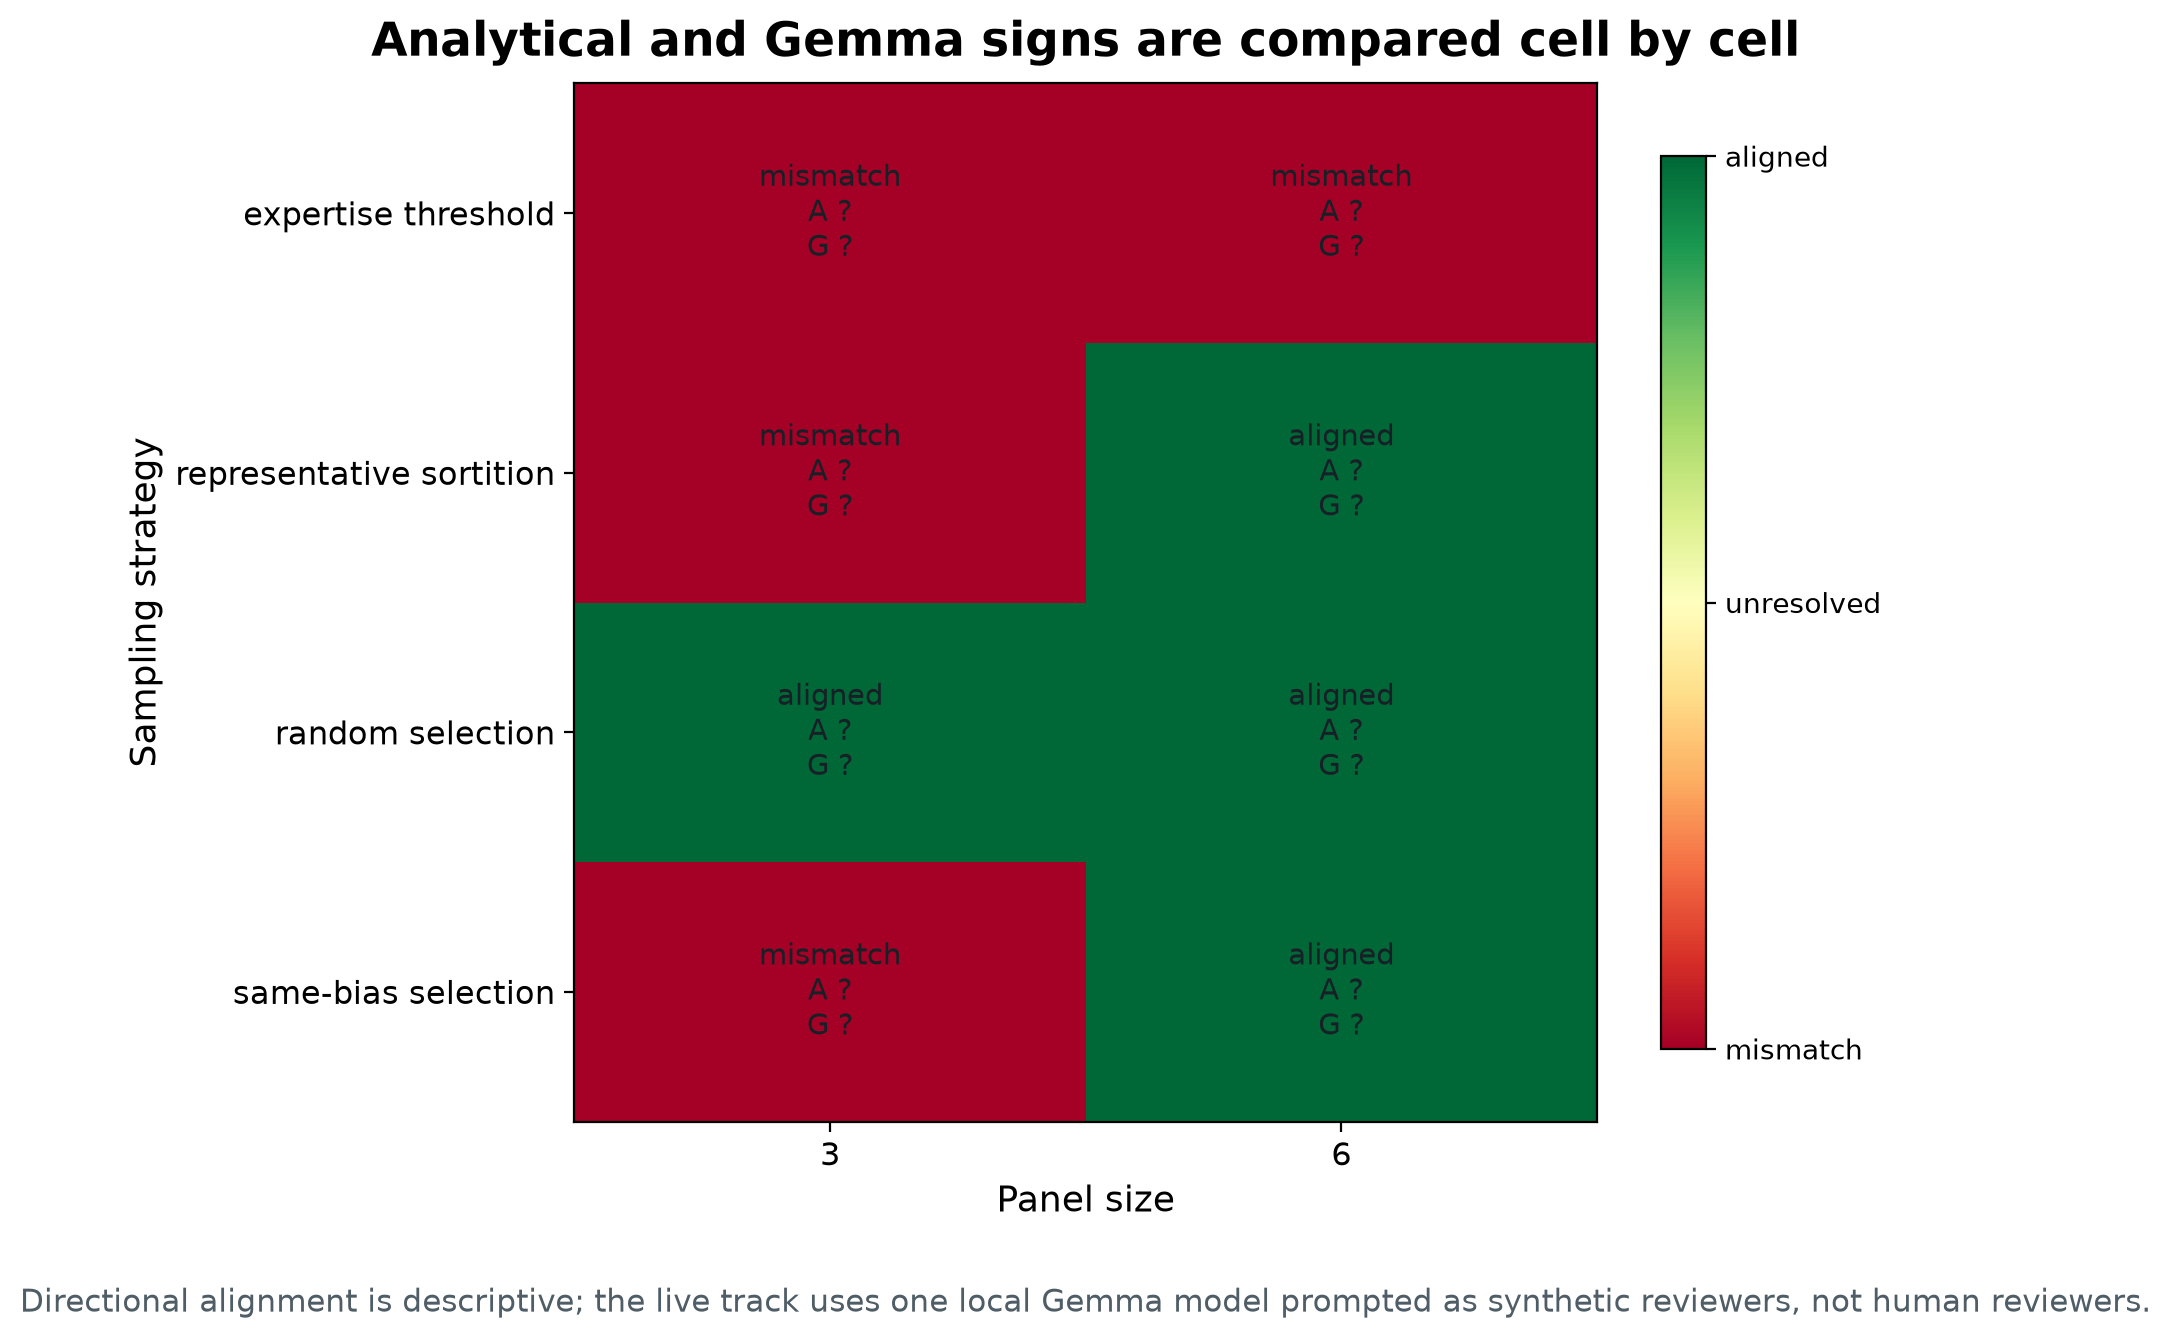
\includegraphics[width=0.72\linewidth,height=0.46\textheight,keepaspectratio,alt={Cell-by-cell alignment grid comparing the analytical age-disparity direction with the live Gemma direction, one cell per strategy x panel-size combination, from source output/data/postdoc\_panel\_alignment.json. Each cell is marked agree, disagree, or unresolved (a zero-sign cell on either track), so the figure functions as the explicit bridge between the controlled and the live track while keeping their uncertainties separate. Statistic: sign agreement between the analytical and live age-disparity directions; resolved-cell agreement 0.500 over 8 resolved cells. Because every live disparity sign is negative in this run, the agreement rate is a weak directional check rather than an independent match, and should be read as such. Claim: the analytical and empirical tracks can be compared cell by cell without pooling their uncertainty; caveat: single-model live evidence is descriptive and n-limited.}]{../figures/postdoc_empirical_alignment.png}
\caption{Cell-by-cell alignment grid comparing the analytical
age-disparity direction with the live Gemma direction, one cell per
strategy x panel-size combination, from source
\protect\breaktt{output/data/postdoc\_panel\_alignment.json}. Each cell
is marked agree, disagree, or unresolved (a zero-sign cell on either
track), so the figure functions as the explicit bridge between the
controlled and the live track while keeping their uncertainties
separate. Statistic: sign agreement between the analytical and live
age-disparity directions; resolved-cell agreement 0.500 over 8 resolved
cells. Because every live disparity sign is negative in this run, the
agreement rate is a weak directional check rather than an independent
match, and should be read as such. Claim: the analytical and empirical
tracks can be compared cell by cell without pooling their uncertainty;
caveat: single-model live evidence is descriptive and
n-limited.}\label{fig:postdocalign}
\end{figure}
\end{block}

\begin{block}{Synthetic strategy ranking does not transfer to the live
track}
\protect\phantomsection\label{synthetic-strategy-ranking-does-not-transfer-to-the-live-track}
\textbf{H5 (does the synthetic ranking transfer to a live single-model
panel?).} The synthetic and live tracks are never pooled, and a
matched-grain comparison shows why pooling would mislead. At the shared
three-seat panel grain (\breakseq{[@fig:trackinversion]}) the strategy
\emph{rank order} inverts between tracks. The rule with by far the
lowest synthetic recovery error --- expertise threshold at 0.037 --- is
the \textbf{worst} under the live Gemma panel at 0.347. The other three
strategies are bunched on \emph{both} tracks --- synthetically at
0.118--0.124 and live at 0.225--0.262 --- so they neither clearly invert
nor clearly transfer. The robust component of the non-transfer is
therefore the expertise-threshold flip alone --- it is the lone clear
outlier on both tracks (best synthetic, worst live) --- so the
non-transfer claim rests on the competence-first rule reversing, not on
a precisely resolved ordering of the other three (which are
statistically indistinguishable on each track). We compare ranks, not
magnitudes, because the two tracks own different oracles and different
uncertainty, so the figure is a qualitative non-transfer result rather
than a pooled effect size.

\begin{figure}
\centering
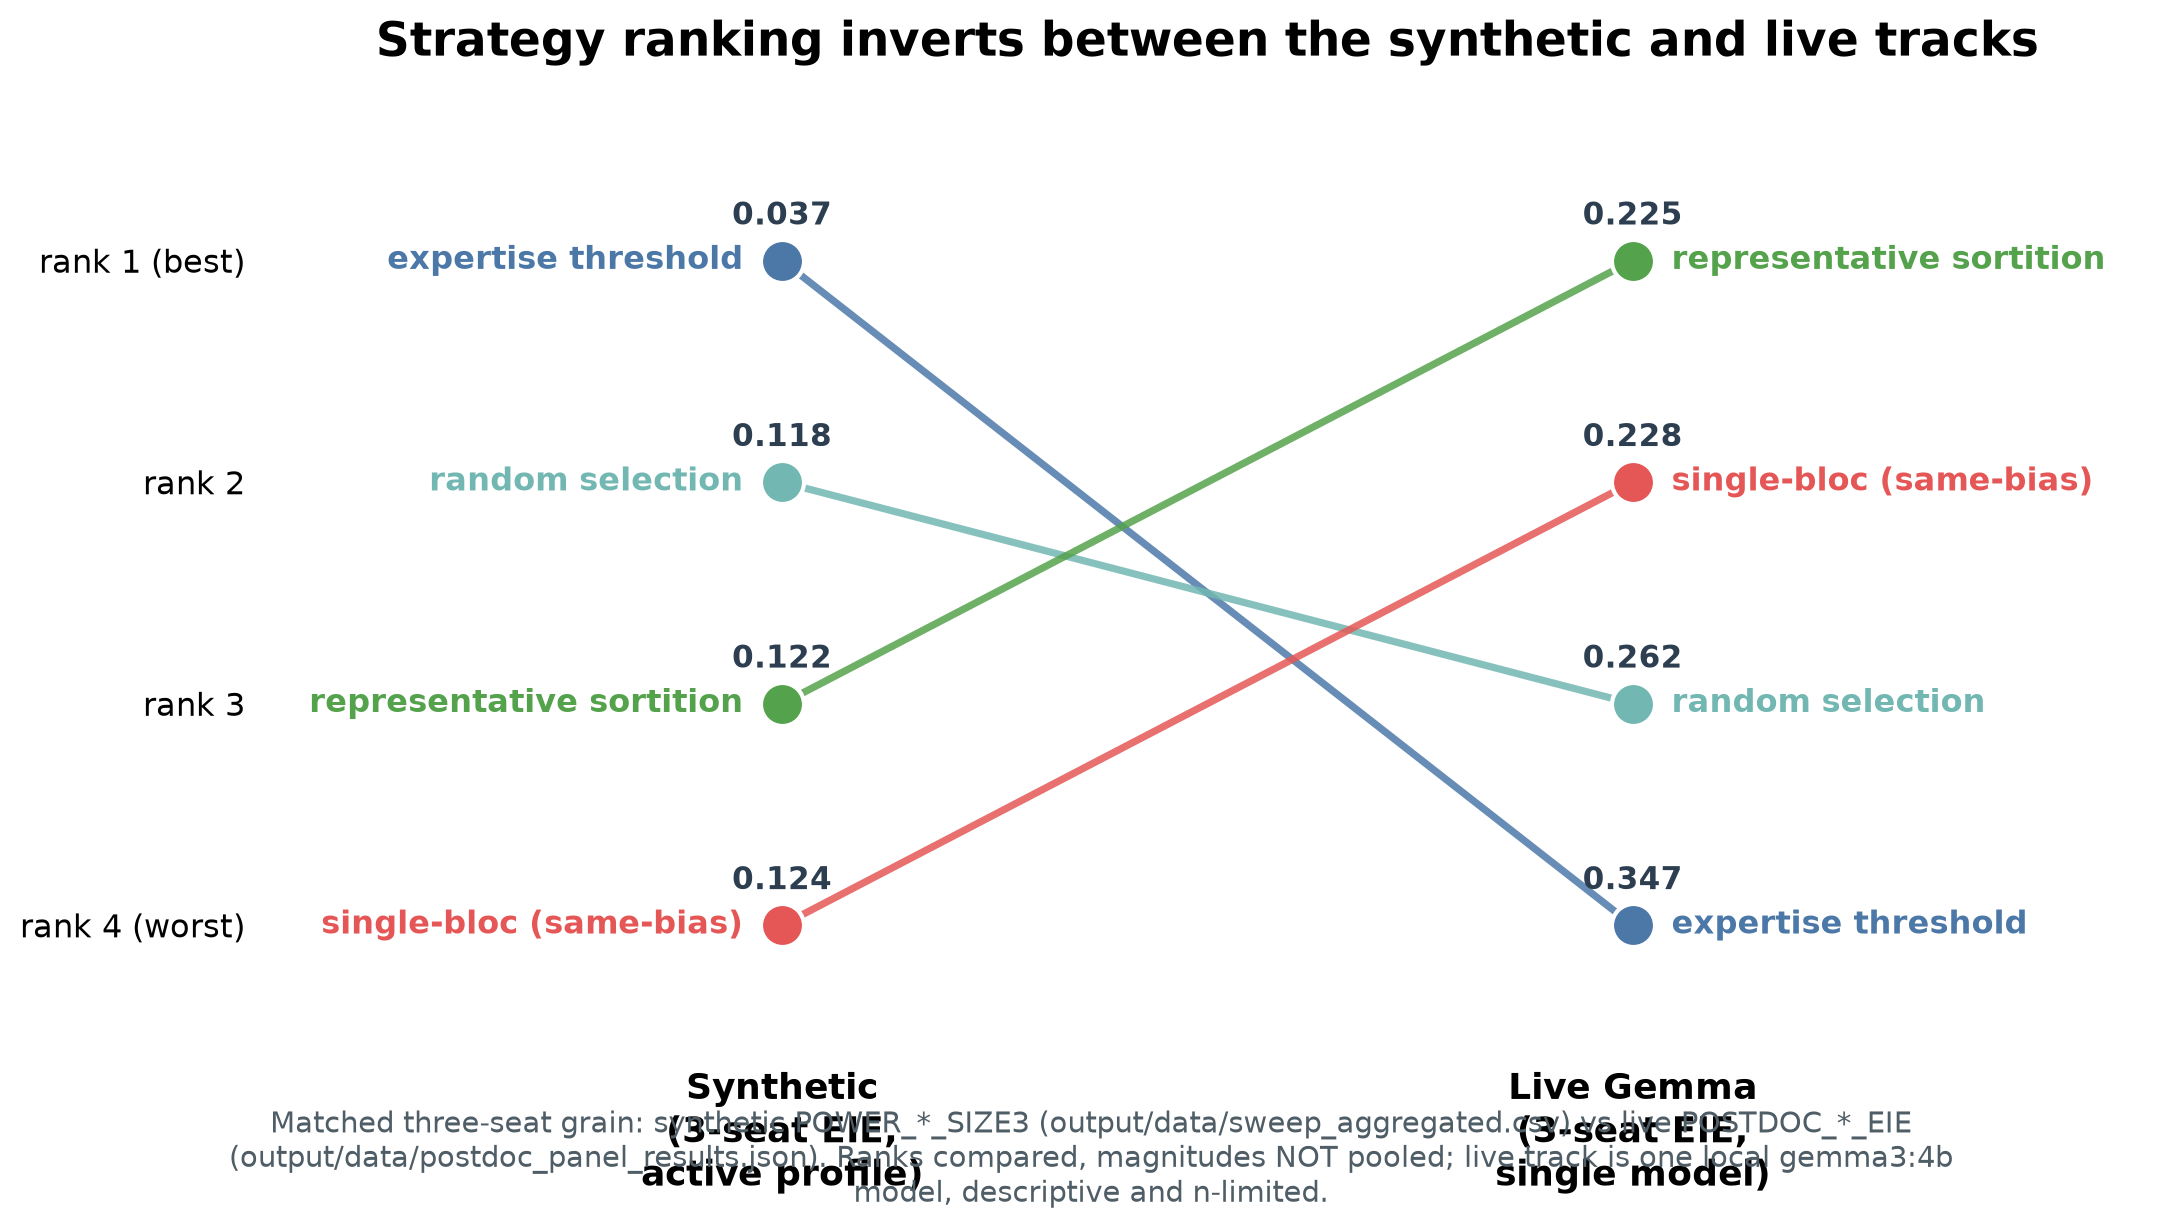
\includegraphics[width=0.8\linewidth,height=0.46\textheight,keepaspectratio,alt={Cross-track strategy-ranking inversion at the matched three-seat grain, shown as a slope chart, from source output/data/sweep\_aggregated.csv (synthetic POWER\_*\_SIZE3, left column) and source output/data/postdoc\_panel\_results.json (live POSTDOC\_*\_EIE, right column). Each strategy is a coloured line connecting its rank under the synthetic track to its rank under the live track; lines that cross are strategies whose standing reverses, and the steepest crossers are expertise threshold (synthetic best to live worst) and single-bloc selection (synthetic worst to live rank-two), while representative sortition is near-best on both tracks. The y-axis is ordinal rank, with the raw error annotated at each node so the reader can see that the live top three are tightly bunched while expertise threshold is the lone outlier. Statistic: ordinal EIE-error rank per track over 96 synthetic seeds and 12 live seeds; ranks compared, magnitudes not pooled (the two tracks own different oracles and uncertainty). Claim: the formation rule that is best blind on synthetic data is worst under one local Gemma model, so the synthetic ranking does not transfer to the live single-model panel; caveat: single-model live evidence is descriptive and n-limited, not a human-review validation.}]{../figures/track_ranking_inversion.png}
\caption{Cross-track strategy-ranking inversion at the matched
three-seat grain, shown as a slope chart, from source
\protect\breaktt{output/data/sweep\_aggregated.csv} (synthetic
\protect\texttt{POWER\_*\_SIZE3}, left column) and source
\protect\breaktt{output/data/postdoc\_panel\_results.json} (live
\protect\texttt{POSTDOC\_*\_EIE}, right column). Each strategy is a
coloured line connecting its rank under the synthetic track to its rank
under the live track; lines that cross are strategies whose standing
reverses, and the steepest crossers are expertise threshold (synthetic
best to live worst) and single-bloc selection (synthetic worst to live
rank-two), while representative sortition is near-best on both tracks.
The y-axis is ordinal rank, with the raw error annotated at each node so
the reader can see that the live top three are tightly bunched while
expertise threshold is the lone outlier. Statistic: ordinal EIE-error
rank per track over 96 synthetic seeds and 12 live seeds; ranks
compared, magnitudes not pooled (the two tracks own different oracles
and uncertainty). Claim: the formation rule that is best blind on
synthetic data is worst under one local Gemma model, so the synthetic
ranking does not transfer to the live single-model panel; caveat:
single-model live evidence is descriptive and n-limited, not a
human-review validation.}\label{fig:trackinversion}
\end{figure}

\textbf{Why the ranking inverts.} The two tracks do genuinely disagree,
and for a principled reason. In the synthetic track the generator
\emph{sets} each judge's accuracy directly, so competence-first
selection seats genuinely higher-accuracy judges and the exact solver
recovers them cleanly --- the ordering is, in part, built into the
data-generating process. Live, ``expertise'' is only a \emph{prompt
instruction}: the local \texttt{gemma3:4b} model need not behave more
accurately, or with more independent errors, when it is told it is an
expert reviewer. Selecting personas by their stated expertise therefore
seats no better live judges, and the rule that wins by construction on
synthetic data carries no guaranteed live advantage --- here it is the
worst. Put differently, the synthetic oracle rewards a property
(controlled judge accuracy) that the prompted model does not inherit
from the persona label. This is a hypothesis about the mechanism, not a
measured causal claim, and it is the empirical reason the manuscript
keeps the synthetic and live tracks at distinct inference levels rather
than reporting a single cross-track strategy winner.
\end{block}
\end{frame}

\end{document}
